\documentclass[10pt,letterpaper]{article}

% --- Paquetes de tipografía, idioma y márgenes ---
\usepackage[utf8]{inputenc}
\usepackage[T1]{fontenc}
\usepackage{lmodern}
\usepackage[letterpaper,top=2.0cm,bottom=2.0cm,left=2.0cm,right=2.0cm]{geometry}

% Configuración manual de títulos en español sin babel
\renewcommand{\contentsname}{Índice General}
\renewcommand{\listtablename}{Índice de Cuadros}
\renewcommand{\listfigurename}{Índice de Figuras}

% --- Paquetes matemáticos y tablas ---
\usepackage{amsmath,amssymb}
\usepackage{booktabs}
\usepackage{tabularx}
\usepackage{xltabular}
\usepackage{pdflscape}
\usepackage{colortbl}
\usepackage{microtype}
\newcolumntype{Y}{>{\centering\arraybackslash}X}
\newcolumntype{L}{>{\raggedright\arraybackslash}X}
\newcolumntype{R}{>{\raggedleft\arraybackslash}X}
\usepackage{array}
\usepackage{xcolor}
\usepackage{graphicx}
\usepackage{float}
\usepackage{fancyhdr}
\usepackage{tcolorbox}
\tcbuselibrary{skins,breakable}
\usepackage{hyperref}
\usepackage{titlesec}
\usepackage{enumitem}
\usepackage{lastpage}
\usepackage{caption}
\captionsetup[table]{name=Cuadro,labelfont=bf,textfont=bf,skip=4pt}
\captionsetup[figure]{name=Figura,labelfont=bf,textfont=bf,skip=4pt}

% Ajuste fino de espaciado en listas
\setlist{nosep,leftmargin=1.5em}
\setlength{\parindent}{0pt}
\setlength{\parskip}{3.5pt}

% --- Definición de Colores Corporativos Solvanta ---
\definecolor{navyblue}{RGB}{26, 79, 124}      % #1a4f7c - Título corporativo y líneas
\definecolor{accentblue}{RGB}{51, 124, 207}   % #337ccf - Subtítulos
\definecolor{darkred}{RGB}{140, 30, 30}       % Puertas de aprobación / límites
\definecolor{tealcolor}{RGB}{30, 110, 110}    % Servicios y variables
\definecolor{forestgreen}{RGB}{20, 120, 40}   % Verificado / Cumplido
\definecolor{boxbg}{RGB}{250, 251, 253}
\definecolor{tableheader}{RGB}{26, 79, 124}
\definecolor{tablerowalt}{RGB}{245, 248, 252}
\definecolor{grayborder}{RGB}{208, 215, 222}

% --- Formato de Secciones con Numeración ---
\titleformat{\section}{\large\bfseries\color{navyblue}}{\thesection.}{0.5em}{}
\titleformat{\subsection}{\normalsize\bfseries\color{navyblue}}{\thesubsection.}{0.5em}{}
\titleformat{\subsubsection}{\small\bfseries\color{accentblue}}{\thesubsubsection.}{0.5em}{}
\titlespacing*{\section}{0pt}{4pt}{2pt}
\titlespacing*{\subsection}{0pt}{3pt}{1pt}
\titlespacing*{\subsubsection}{0pt}{2pt}{1pt}

% --- Formato de Encabezados y Pies de Página ---
\pagestyle{fancy}
\fancyhf{}
\lhead{\small\color{navyblue}\textbf{Solvanta Engineering Solutions} \textbar\ DPyPQ}
\rhead{\small Documento Técnico LE-01 \textbar\ Lista Maestra de Equipos y DFP v1}
\cfoot{\small Página \thepage\ de \pageref{LastPage}}
\renewcommand{\headrulewidth}{0.4pt}
\renewcommand{\footrulewidth}{0pt}
\setlength{\headheight}{14pt}

% --- Cajas Estilizadas tcolorbox ---
\newtcolorbox{propositobox}{
    colframe=navyblue,
    colbacktitle=navyblue,
    coltitle=white,
    fonttitle=\bfseries\small,
    title=Propósito de la Actividad de Ingeniería LE-01,
    colback=white,
    arc=1.5mm,
    boxrule=0.7pt,
    titlerule=0pt,
    left=3.0mm, right=3.0mm, top=2.0mm, bottom=2.0mm
}

\hypersetup{
    colorlinks=true,
    linkcolor=navyblue,
    citecolor=navyblue,
    urlcolor=accentblue,
    pdfauthor={Solvanta Engineering Solutions S.A. de C.V.},
    pdftitle={LE-01_Solvanta: Lista Maestra de Equipos y Variables de Proceso}
}

\begin{document}

% ==============================================================================
% PORTADA CORPORATIVA OFICIAL
% ==============================================================================
\begin{titlepage}
    \centering
    
\includegraphics[width=0.28\textwidth]{logo_empresa.png}\\[0.4cm]
    {\scshape\Large Benemérita Universidad Autónoma de Puebla}\\[0.15cm]
    {\scshape\large Facultad de Ingeniería Química \textbar\ Colegio de Ingeniería Química}\\[0.15cm]
    {\large Diseño de Procesos y Productos Químicos (DPyPQ)}\\[0.1cm]
    {\small Catedrático: Dr. Jesús Andrés Arzola Flores}\\[0.6cm]

    \hrule height 2pt
    \vspace{0.4cm}
    {\LARGE \bfseries \color{navyblue} ACTIVIDAD LE-01: LISTA MAESTRA DE EQUIPOS Y VARIABLES DE DISEÑO DE PROCESO}\\[0.3cm]
    {\Large \bfseries Integración de Balances de Materia/Energía y Elaboración del Diagrama de Flujo de Proceso (DFP v1 / Rev. 1)}\\[0.3cm]
    {\large \textbf{Proyecto:} Planta de Producción de e-Metanol Grado AA ($30\,000\text{ t/año}$) a partir de $\text{CO}_2$ Capturado e $\text{H}_2$ Verde Vía Electrólisis SOEC de Alta Temperatura}\\[0.4cm]
    \hrule height 1pt
    \vspace{0.6cm}

    \begin{tcolorbox}[colframe=navyblue,colback=boxbg,arc=2mm,boxrule=0.8pt]
        \centering
        {\LARGE \textbf{\color{navyblue} SOLVANTA ENGINEERING SOLUTIONS S.A. DE C.V.}}\\[0.2cm]
        \small \textbf{Código del Documento Oficial:} \texttt{LE-01\_Solvanta.pdf} \textbar\ \textbf{Entregable Fase 2:} \texttt{E2.1\_DOC\_ListaEquipos\_v1.0.pdf}\\
        \textbf{Código del Diagrama Asociado:} \texttt{DFP-v1\_Solvanta.pdf} \textbar\ \textbf{Revisión:} 1.0 (Definitiva / Aprobada para Diseño Básico)\\
        \textbf{Fecha de Emisión:} 21 de Septiembre de 2026 \textbar\ \textbf{Ubicación de Planta:} Complejo Petroquímico Cangrejera, Coatzacoalcos, Ver.
    \end{tcolorbox}

    \vspace{0.4cm}
    \begin{tcolorbox}[colframe=navyblue,colback=white,arc=2mm,boxrule=0.8pt]
        \centering
        \textbf{\color{navyblue}\large Repositorio Oficial del Proyecto en GitHub}\\[3pt]
        \href{https://github.com/karolcamachol29-sudo/RFP-CCM-EM-001}{\texttt{\textbf{https://github.com/karolcamachol29-sudo/RFP-CCM-EM-001}}}\\[4pt]
        \footnotesize
        \textbf{Rama:} \texttt{main} \quad $\bullet$ \quad
        \textbf{Licitación:} \texttt{RFP-CCM-EM-001} \quad $\bullet$ \quad
        \textbf{Directorio del Entregable:} \texttt{03\_Entregables\_Finales/E2/LE-01\_Solvanta/}
    \end{tcolorbox}

    \vspace{0.4cm}
    \textbf{\large EQUIPO DE TRABAJO Y DIRECCIÓN TÉCNICA:}\\[0.25cm]
    \begin{center}
    \footnotesize
    \setlength{\tabcolsep}{4pt}
    \begin{tabularx}{\textwidth}{>{\bfseries}p{4.3cm} X >{\centering\arraybackslash}p{2.4cm} >{\centering\arraybackslash}p{2.6cm}}
        \toprule
        \textbf{Puesto en la Empresa} & \textbf{Ingeniero(a) Responsable} & \textbf{Matrícula / ID} & \textbf{Usuario GitHub} \\
        \midrule
        Directora de Proyecto, Python y Optimización & Ing. Karol Paola Camacho López & FIQ--BUAP & \texttt{@Karoc} \\
        Simulación DWSIM e Instrumentación & Ing. Paulina Mota Macip & FIQ--BUAP & \texttt{@paulina145} \\
        Ing. de Procesos, Plant 3D y DFP v1 & Ing. Gildardo Ocaña Barrales & FIQ--BUAP & \texttt{@GildardoOca25} \\
        Evaluación Económica (BioSTEAM) y HSE & Ing. Grecia Figueroa Rincón & FIQ--BUAP & \texttt{@Cho0bb} \\
        \bottomrule
    \end{tabularx}
    \end{center}

    \vfill
    {\footnotesize Puebla, Pue. \textbar\ Ciclo Otoño 2026 \textbar\ Solvanta Engineering Solutions S.A. de C.V. \copyright\ Todos los derechos reservados.}
\end{titlepage}

% ==============================================================================
% CONTROL DE VERSIONES Y REGISTRO DE CAMBIOS
% ==============================================================================
\section*{Control de Revisiones del Documento}
\addcontentsline{toc}{section}{Control de Revisiones del Documento}

\begin{table}[H]
\centering
\small
\begin{tabularx}{\textwidth}{c c c X c}
\toprule
\textbf{Rev.} & \textbf{Fecha} & \textbf{Elaboró} & \textbf{Descripción del Cambio / Alcance} & \textbf{Aprobó} \\
\midrule
0.1 & 14/09/2026 & Equipo Solvanta & Borrador preliminar de lista de equipos y asignación inicial de TAGs preliminares. & Dir. Técnica \\
0.2 & 18/09/2026 & Ing. Simulación & Incorporación de balances de materia TC-01 y energía TE-01 convergidos en DWSIM v1. & Líder Proceso \\
\bottomrule
\end{tabularx}
\end{table}

\vspace{0.2cm}
\tableofcontents
\vspace{0.3cm}
\listoftables
\vspace{0.3cm}
\listoffigures
\newpage

% ==============================================================================
% SECCIÓN 1: INTRODUCCIÓN Y PROPÓSITO DE LA ACTIVIDAD
% ==============================================================================
\section{Introducción y Propósito de la Actividad de Ingeniería LE-01}

La transición entre la etapa de simulación termodinámica rigurosa (Fase 1: Verificación Termodinámica de Proceso VTP-01) y la fase de diseño básico de ingeniería (Fase 2) exige formalizar la arquitectura global de la planta. Mientras que el modelo computacional implementado en \texttt{DWSIM v10.2.4} resuelve los balances de materia y energía punto a punto, las herramientas de simulación suelen incorporar bloques matemáticos abstractos (tales como divisores ideales, multiplicadores de corriente, reactores de conversión estequiométrica ideal o separadores por componentes) que carecen de correspondencia unívoca en el mundo industrial.

\begin{propositobox}
El propósito técnico de la \textbf{Actividad LE-01} consiste en:
\begin{enumerate}[leftmargin=*]
    \item Transformar la simulación convergida \texttt{DWSIM v1} en una estructura industrialmente realizable mediante la emisión del \textbf{Diagrama de Flujo de Proceso v1 (DFP v1 / Rev. 1)}.
    \item Generar la \textbf{Lista Maestra de Equipos (LE-01C)}, asignando a cada unidad un identificador alfanumérico único (TAG) conforme a estándares internacionales (ANSI/ISA-5.1 y normas de referencia PEMEX NRF-048).
    \item Consolidar las \textbf{Condiciones Normales de Operación (LE-01D)}, garantizando coherencia absoluta con las tablas maestras de materia (\texttt{TC-01}) y energía (\texttt{TE-01}).
    \item Identificar, jerarquizar y delimitar las \textbf{Variables de Diseño de Proceso (LE-01E)} y sus relaciones directas con los \textbf{Indicadores Clave de Desempeño (LE-01F)}.
    \item Documentar la trazabilidad técnica de las decisiones de proceso basadas en los \textbf{Análisis de Sensibilidad (LE-01G y LE-01H)}, la selección de \textbf{Alternativas Tecnológicas (LE-01I)}, los \textbf{Supuestos Críticos (LE-01K)} y la matriz de \textbf{Información Pendiente (LE-01J)}.
\end{enumerate}
\end{propositobox}

\textbf{Solvanta Engineering Solutions S.A. de C.V.} desarrolló el proyecto de diseño básico para la producción de $\mathbf{30\,000\text{ t/año}}$ ($\mathbf{3\,788.65\text{ kg/h}}$ continuos con factor de servicio de $8\,000\text{ h/año}$) de e-metanol con pureza comercial Grado AA ($>99.85\%$ p/p). La instalación se ubica estratégicamente en el Complejo Petroquímico Cangrejera (Coatzacoalcos, Veracruz), aprovechando la disponibilidad de dióxido de carbono capturado de alta pureza ($99.0\%$ molar) procedente de unidades petroquímicas y fuentes de energía renovable para la generación de hidrógeno verde mediante electrólisis de óxido sólido a alta temperatura (SOEC).

% ==============================================================================
% SECCIÓN 2: MARCO CONCEPTUAL Y ABREVIATURAS (CUADRO 1)
% ==============================================================================
\section{Marco Conceptual y Abreviaturas Utilizadas en la Actividad}

Para garantizar un lenguaje técnico homogéneo y libre de ambigüedades a lo largo de todo el expediente de ingeniería, se definen los acrónimos utilizados en el proceso en el Cuadro \ref{tab:cuadro1}.

\begin{table}[H]
\centering
\small
\caption{\textbf{Abreviaturas y acrónimos técnicos utilizados en la actividad.}} \label{tab:cuadro1}
\begin{tabularx}{\textwidth}{l p{4.2cm} l p{5.5cm}}
\toprule
\textbf{Acrónimo} & \textbf{Significado Técnico} & \textbf{Acrónimo} & \textbf{Significado Técnico} \\
\midrule
\textbf{ANSI} & American National Standards Institute & \textbf{LHV} & Lower Heating Value (Poder Calorífico Inf.) \\
\textbf{API} & American Petroleum Institute & \textbf{M} & Módulo Estequiométrico Syngas $((H_2-CO_2)/(CO+CO_2))$ \\
\textbf{ASME} & American Society of Mechanical Engineers & \textbf{MeOH} & Metanol ($\text{CH}_3\text{OH}$) Grado AA \\
\textbf{BWR} & Boiling Water Reactor (Reactor Carcasa-Tubos) & \textbf{PEM} & Proton Exchange Membrane (Electrólisis) \\
\textbf{DFP / PFD} & Diagrama de Flujo de Proceso & \textbf{PRSV2-VL} & Peng-Robinson-Stryjek-Vera Modificado \\
\textbf{DWSIM} & Simulador de Procesos Químicos Open-Source & \textbf{P\&ID} & Diagrama de Tubería e Instrumentación \\
\textbf{E2} & Fase 2: Ingeniería Básica y Lista de Equipos & \textbf{RWGS} & Reverse Water Gas Shift ($\text{CO}_2 + \text{H}_2 \leftrightarrow \text{CO} + \text{H}_2\text{O}$) \\
\textbf{FEHE} & Feed/Effluent Heat Exchanger (Economizador) & \textbf{SOEC} & Solid Oxide Electrolysis Cell (Electrólisis a vapor) \\
\textbf{HP / LP} & High Pressure (Alta P.) / Low Pressure (Baja P.) & \textbf{TAG} & Etiqueta Alfanumérica Única de Identificación \\
\textbf{ID} & Indicador de Desempeño Técnico (KPI) & \textbf{VTP} & Verificación Termodinámica de Proceso \\
\textbf{ISA} & International Society of Automation & \textbf{ZLD} & Zero Liquid Discharge (Descarga Líquida Cero) \\
\bottomrule
\end{tabularx}
\end{table}

% ==============================================================================
% SECCIÓN 3: DISTRIBUCIÓN DEL TRABAJO DURANTE LA SEMANA (CUADRO 2)
% ==============================================================================
\section{Distribución del Trabajo Técnico durante la Semana de Ejecución}

Para dar cumplimiento a la metodología de aseguramiento de calidad de Solvanta Engineering Solutions y asegurar una revisión cruzada exhaustiva antes del cierre del entregable, las actividades de la semana fueron estructuradas conforme al Cuadro \ref{tab:cuadro2}.

\begin{table}[H]
\centering
\small
\setlength{\tabcolsep}{4pt}
\caption{\textbf{Distribución del trabajo técnico y cronograma semanal de la firma Solvanta.}} \label{tab:cuadro2}
\begin{tabularx}{\textwidth}{c p{3.0cm} X p{3.6cm} c}
\toprule
\textbf{Día} & \textbf{Etapa Metodológica} & \textbf{Actividades Clave Desarrolladas} & \textbf{Responsable Principal} & \textbf{Estado} \\
\midrule
\textbf{Día 1} & Revisión DFP v0 y Delimitación & Evaluación formal del plano preliminar DFP v0, delimitación de límites de batería de los 7 sistemas de proceso (Cuadros LE-01A y LE-01B). & Ing. Gildardo Ocaña Barrales (Ing. Procesos / Plant 3D) & \textbf{100\%} \\
\textbf{Día 2} & Lista Maestra y TAGs & Inventario de las 28 unidades físicas del proceso, eliminación de objetos matemáticos de DWSIM, asignación formal de TAGs únicos (Cuadro LE-01C). & Ing. Gildardo Ocaña Barrales \& Ing. Karol Camacho & \textbf{100\%} \\
\textbf{Día 3} & Condiciones de Operación & Calibración termodinámica rigurosa de cada equipo contra las tablas oficiales de materia TC-01 y energía TE-01 de DWSIM v1 (Cuadro LE-01D). & Ing. Paulina Mota Macip (Simulación DWSIM) & \textbf{100\%} \\
\textbf{Día 4} & Variables e Indicadores & Identificación de 10 variables de proceso críticas, rangos operativos admisibles, cálculo de KPIs y márgenes de diseño (Cuadros LE-01E y LE-01F). & Ing. Karol Paola Camacho López (Dirección Proyecto) & \textbf{100\%} \\
\textbf{Día 5} & Sensibilidad y Alternativas & Integración de estudios de sensibilidad de síntesis y separación, matriz de trazabilidad y evaluación de tecnologías (Cuadros LE-01G, LE-01H y LE-01I). & Ing. Paulina Mota Macip \& Ing. Gildardo Ocaña & \textbf{100\%} \\
\textbf{Día 6} & Supuestos y Verificación & Declaración de supuestos de base, matriz de información pendiente hacia E2 y verificación integral del plano DFP v1 (Cuadros LE-01J, LE-01K y 15). & Ing. Grecia Figueroa Rincón (HSE y Calidad) & \textbf{100\%} \\
\textbf{Día 7} & Cierre y Compilación & Redacción de conclusiones técnicas (Sec. 18), respuestas al cuestionario (Sec. 20), compilación en LaTeX y emisión del paquete de entrega. & Ing. Karol Paola Camacho López (Dirección Técnica) & \textbf{100\%} \\
\bottomrule
\end{tabularx}
\end{table}

\newpage
% ==============================================================================
% SECCIÓN 4: ETAPA 1. REVISIÓN Y EVALUACIÓN DEL DFP v0 (CUADRO 3: LE-01A)
% ==============================================================================
\section{Etapa 1. Revisión y Evaluación Técnica del DFP v0 (Cuadro 3: LE-01A)}

Antes de consolidar el plano de ingeniería definitiva DFP v1, la firma efectuó una auditoría crítica sobre el diagrama preliminar DFP v0 generado al inicio del proyecto. El objetivo de esta etapa fue detectar deficiencias de representación, inconsistencias de conectividad y la presencia de abstracciones matemáticas de la herramienta de simulación.

\begin{table}[H]
\centering
\small
\caption{\textbf{LE-01A. Revisión y auditoría técnica del DFP v0.}} \label{tab:cuadro3}
\begin{tabularx}{\textwidth}{c p{5.5cm} c X}
\toprule
\textbf{Núm.} & \textbf{Criterio de Evaluación Técnica} & \textbf{Cumple} & \textbf{Evidencia u Observación de la Firma Solvanta} \\
\midrule
1 & Todos los equipos tienen un TAG único y normalizado. & \textbf{Sí} & En DFP v0 algunos equipos compartían etiquetas genéricas (ej. \texttt{MIX-1}, \texttt{HE-1}). Se normalizó a estándar ANSI/ISA (\texttt{MIX-301}, \texttt{E-501}, \texttt{R-401}). \\
2 & Las corrientes de proceso siguen un orden secuencial y coherente. & \textbf{Sí} & Las corrientes de materia fueron renumeradas secuencialmente por áreas de proceso (\texttt{S-101} a \texttt{S-804}), coincidiendo 100\% con la tabla de corrientes \texttt{TC-01}. \\
3 & Se identifican claramente los límites de batería y servicios. & \textbf{Sí} & Se agregaron banderas de entrada para $\text{CO}_2$, agua cruda, vapor de calentamiento, agua de enfriamiento (CW) y conexiones al lazo ZLD. \\
4 & Los balances de materia y energía son representables físicamente. & \textbf{Sí} & Se verificó que ninguna corriente contenga temperaturas cruzadas imposibles; el economizador FEHE \texttt{E-502A/B} respeta un $\Delta T_{\text{pinch}} \ge 20^\circ\text{C}$. \\
5 & La recirculación de gas no convertido se representa explícitamente. & \textbf{Sí} & Se representó el bucle cerrado desde el flash \texttt{V-501}, pasando por el divisor \texttt{SPLIT-501}, soplador \texttt{C-501} y reingreso al mezclador \texttt{MIX-401}. \\
6 & Se eliminaron los bloques puramente matemáticos del simulador. & \textbf{Sí} & Se sustituyó el separador por componentes \texttt{SEP-01} de DWSIM por una columna fraccionadora de destilación real \texttt{T-601} con condensador y rehervidor. \\
7 & Se incluyeron las corrientes de purga requeridas para evitar acumulación. & \textbf{Sí} & Se incorporó formalmente la corriente de purga \texttt{S-505} (4.0\% del gas de reciclo), acoplándola a un turboexpansor de recuperación \texttt{EXP-501}. \\
8 & El cajetín incluye metadatos de ingeniería completos y aprobaciones. & \textbf{Sí} & Se incluyó cajetín oficial con fecha (21/09/2026), número de revisión (Rev. 1), escala, título corporativo y firmas de responsabilidad técnica. \\
\bottomrule
\end{tabularx}
\end{table}

% ==============================================================================
% SECCIÓN 5: ETAPA 2. DELIMITACIÓN DE SISTEMAS Y LÍMITES DE PROCESO (CUADRO 4: LE-01B)
% ==============================================================================
\section{Etapa 2. Delimitación de Sistemas del Proceso (Cuadro 4: LE-01B)}

Para organizar modularmente la planta y permitir la distribución paralela de actividades de ingeniería de detalle, la planta de e-metanol se subdividió en 7 áreas o sistemas de proceso interconectados (Cuadro \ref{tab:cuadro4}).

\begin{table}[H]
\centering
\small
\caption{\textbf{LE-01B. Límites de los sistemas y áreas del proceso Solvanta.}} \label{tab:cuadro4}
\begin{tabularx}{\textwidth}{c p{2.2cm} p{1.8cm} p{3.0cm} p{2.2cm} X}
\toprule
\textbf{Sistema} & \textbf{Nombre del Área} & \textbf{TAGs Principales} & \textbf{Incluye} & \textbf{No Incluye} & \textbf{Justificación de Límites} \\
\midrule
\textbf{Área 100} & Recepción y Acond. de $\text{CO}_2$ & \texttt{C-101}, \texttt{E-101}, \texttt{V-101} & Compresión desde $1.013$ a $20\text{ bar}$, enfriamiento y separación de condensados. & Planta de captura externa de $\text{CO}_2$. & Garantiza entrega de $\text{CO}_2$ seco a la misma presión de salida de la electrólisis SOEC. \\
\textbf{Área 200} & Generación de $\text{H}_2$ Verde (SOEC) & \texttt{P-201}, \texttt{MIX-201}, \texttt{E-202}, \texttt{EL-201}, \texttt{E-201}, \texttt{E-203}, \texttt{V-201} & Bombeo de agua, sobrecalentamiento a $750^\circ\text{C}$, celdas SOEC, enfriamiento y separación $\text{H}_2/\text{H}_2\text{O}$. & Planta de purificación de agua desmineralizada de red. & Agrupa la tecnología electroquímica a alta temperatura y el acondicionamiento de $\text{H}_2$ a $19.4\text{ bar}$. \\
\textbf{Área 300} & Compresión y Mezcla de Syngas & \texttt{MIX-301}, \texttt{E-301}, \texttt{C-301} & Mezclador estático de gases frescos, precalentador a succión y compresor centrífugo a $75\text{ bar}$. & Bucle de reciclo de alta presión. & Eleva la presión de reactivos estequiométricos ($M=2.05$) a la presión óptima de síntesis. \\
\textbf{Área 400} & Síntesis Catalítica de Metanol & \texttt{MIX-401}, \texttt{E-502A/B}, \texttt{R-401}, \texttt{R-401-S} & Mezcla con reciclo, precalentamiento FEHE, reactor multitubular Lurgi BWR y generación de vapor. & Separación de productos condensados. & Contiene la reacción exotérmica principal ($\text{CO}_2+3\text{H}_2 \leftrightarrow \text{CH}_3\text{OH}+\text{H}_2\text{O}$) y el vapor acoplado a SOEC. \\
\textbf{Área 500} & Condensación, Flash y Reciclo & \texttt{E-501}, \texttt{V-501}, \texttt{SPLIT-501}, \texttt{C-501}, \texttt{EXP-501} & Condensador principal a $38^\circ\text{C}$, tambor flash HP a $75\text{ bar}$, división de purga, soplador y turboexpansor. & Destilación fraccionada de metanol. & Maximiza la recuperación de metanol bruto líquido ($99.85\%$) y retorna reactivos gaseosos no convertidos. \\
\textbf{Área 600} & Purificación y Destilación MeOH & \texttt{V-601}, \texttt{P-601}, \texttt{T-601}, \texttt{E-601}, \texttt{E-602}, \texttt{E-603}, \texttt{TK-601} & Desgasificador LP a $1.25\text{ bar}$, columna de destilación de 32 etapas, condensador, rehervidor y tanque. & Tratamiento de efluentes de fondo. & Separa metanol puro comercial Grado AA ($99.89\%$ p/p) del agua de reacción. \\
\textbf{Área 800} & Circuito Hídrico ZLD y Auxiliares & \texttt{P-801}, \texttt{FL-801}, Torres Enfriam. & Recolección de condensados SOEC y fondos de destilación, filtración y recirculación a caldera. & Manejo de sólidos o lodos deshidratados. & Cierra el ciclo hidrológico de planta evitando descarga de efluentes líquidos al ambiente. \\
\bottomrule
\end{tabularx}
\end{table}

\newpage
% ==============================================================================
% SECCIÓN 6: ETAPA 3. SISTEMA DE ASIGNACIÓN DE TAGS (CUADRO 5)
% ==============================================================================
\section{Etapa 3. Sistema de Asignación de TAGs (Cuadro 5)}

La codificación de cada unidad física sigue el estándar normalizado \texttt{[PREFIJO]-[ÁREA][CONSECUTIVO]} (Cuadro \ref{tab:cuadro5}), garantizando unicidad y rápida identificación en campo.

\begin{table}[H]
\centering
\small
\caption{\textbf{Nomenclatura normalizada para asignación de TAGs en la planta Solvanta.}} \label{tab:cuadro5}
\begin{tabularx}{\textwidth}{c l X p{4.2cm}}
\toprule
\textbf{Prefijo} & \textbf{Familia de Equipo} & \textbf{Descripción Funcional} & \textbf{Ejemplos en Planta Solvanta} \\
\midrule
\textbf{C} & Compresores / Sopladores & Elevación de presión de corrientes gaseosas y recirculación & \texttt{C-101}, \texttt{C-301}, \texttt{C-501} \\
\textbf{E} & Intercambiadores de Calor & Calentadores, enfriadores, condensadores, rehervidores y FEHE & \texttt{E-101}, \texttt{E-202}, \texttt{E-203}, \texttt{E-301}, \texttt{E-501}, \texttt{E-601} \\
\textbf{EL / SOEC} & Paquete de Electrólisis & Módulos de celdas de disociación de vapor de agua a alta $T$ & \texttt{EL-201} (\texttt{SOEC-201}) \\
\textbf{EXP / X} & Turboexpansores & Máquinas de expansión isentrópica para recuperación de potencia & \texttt{EXP-501} (\texttt{X-501}) \\
\textbf{MIX} & Mezcladores Estáticos & Unión física de corrientes de reactivos, reciclos o agua & \texttt{MIX-201}, \texttt{MIX-301}, \texttt{MIX-401} \\
\textbf{P} & Bombas Centrífugas & Impulsión de líquidos presurizados (make-up, reflujo, fondos) & \texttt{P-201}, \texttt{P-601}, \texttt{P-801} \\
\textbf{R} & Reactores Químicos & Vasos de reacción con lecho catalítico y remoción térmica & \texttt{R-401} (con carcasa \texttt{R-401-S}) \\
\textbf{SPLIT} & Divisores de Flujo & Desvío de fracciones controladas para purga de incondensables & \texttt{SPLIT-501} \\
\textbf{T} & Columnas de Separación & Torres fraccionadoras de platos o empaque para purificación & \texttt{T-601} (Columna de Destilación) \\
\textbf{TK} & Tanques de Almacenamiento & Recipientes atmosféricos o presurizados para acumulación & \texttt{TK-601} (Metanol comercial) \\
\textbf{V} & Recipientes / Separadores & Tambores de separación gas-líquido tipo Knock-Out y flash & \texttt{V-101}, \texttt{V-201}, \texttt{V-501}, \texttt{V-601} \\
\bottomrule
\end{tabularx}
\end{table}

% ==============================================================================
% SECCIÓN 7: ETAPA 4. LISTA MAESTRA DE EQUIPOS (CUADRO 6: LE-01C)
% ==============================================================================
\begin{landscape}
\section{Etapa 4. Lista Maestra de Equipos de Proceso (Cuadro 6: LE-01C)}

A continuación se presenta el inventario completo de los \textbf{28 equipos de proceso} que conforman la planta de e-metanol Solvanta. Cada equipo cuenta con función técnica definida, asignación unívoca de corrientes de entrada/salida y variable principal de control de proceso.

\setlength{\tabcolsep}{3.5pt}
\small
\begin{xltabular}{\linewidth}{l >{\raggedright\arraybackslash}p{3.2cm} >{\raggedright\arraybackslash}X >{\centering\arraybackslash}p{2.0cm} >{\centering\arraybackslash}p{2.2cm} >{\raggedright\arraybackslash}p{4.5cm} c}
\caption{\textbf{LE-01C. Lista maestra de equipos de proceso de la planta Solvanta.}} \label{tab:cuadro6} \\
\toprule
\textbf{TAG} & \textbf{Equipo u Operación} & \textbf{Función de Proceso} & \textbf{Entradas} & \textbf{Salidas} & \textbf{Variable Principal de Diseño} & \textbf{Estado} \\
\midrule
\endfirsthead
\toprule
\textbf{TAG} & \textbf{Equipo u Operación} & \textbf{Función de Proceso} & \textbf{Entradas} & \textbf{Salidas} & \textbf{Variable Principal de Diseño} & \textbf{Estado} \\
\midrule
\endhead
\bottomrule
\multicolumn{7}{r}{\footnotesize\textit{Continúa en la siguiente página\dots}} \\
\endfoot
\bottomrule
\endlastfoot
\texttt{C-101} & Compresor de $\text{CO}_2$ de Captura & Elevar presión de $\text{CO}_2$ capturado de $1.013$ a $20.0\text{ bar}$. & \texttt{S-100} & \texttt{S-101A} & Presión de descarga y potencia ($W=285.5\text{ kW}$). & Definido \\
\texttt{E-101} & Interenfriador de $\text{CO}_2$ & Enfriar el $\text{CO}_2$ comprimido de $115^\circ\text{C}$ a $25^\circ\text{C}$ con agua de servicio. & \texttt{S-101A} & \texttt{S-101B} & Temperatura de salida ($25^\circ\text{C}$) y carga térmica. & Definido \\
\texttt{V-101} & Separador Knock-Out $\text{CO}_2$ & Remover condensados de agua arrastrados en el $\text{CO}_2$ frío. & \texttt{S-101B} & \texttt{S-101}, \texttt{S-COND} & Eficiencia de separación de niebla y nivel. & Definido \\
\texttt{P-201} & Bomba de Agua Make-up & Presurizar agua fresca de red de $1.013$ a $20.0\text{ bar}$ hacia la caldera. & \texttt{S-200} & \texttt{S-201} & Altura manométrica ($H=195\text{ m}$) y caudal volumétrico. & Definido \\
\texttt{MIX-201} & Mezclador de Agua a Caldera & Combinar agua fresca de make-up con agua recuperada ZLD. & \texttt{S-201}, \texttt{S-202} & \texttt{S-203} & Temperatura de mezcla resultante ($39.8^\circ\text{C}$). & Definido \\
\texttt{R-401-S} & Caldera BWR Generadora de Vapor & Generar vapor saturado a $20.0\text{ bar}$ usando calor exotérmico del reactor. & \texttt{S-203} & \texttt{S-204} & Carga térmica transferida ($Q=12\,335.4\text{ kW}$) a $220^\circ\text{C}$. & Definido \\
\texttt{E-202} & Sobrecalentador Eléctrico Vapor & Sobrecalentar vapor de $220^\circ\text{C}$ a $750^\circ\text{C}$ para alimentación a SOEC. & \texttt{S-204} & \texttt{S-205} & Temperatura de entrada a celdas SOEC ($750^\circ\text{C}$). & Definido \\
\texttt{EL-201} & Stack Electrolizador SOEC & Disociar vapor de agua al $70\%$ a $750^\circ\text{C}$ produciendo $\text{H}_2$ y $\text{O}_2$. & \texttt{S-205} & \texttt{S-206}, \texttt{S-207} & Consumo de potencia eléctrica ($54\,402\text{ kW}$) y conversión. & Definido \\
\texttt{E-201} & Recuperador Enfriador de $\text{O}_2$ & Enfriar oxígeno puro subproducto de $750^\circ\text{C}$ a $31^\circ\text{C}$. & \texttt{S-206} & \texttt{S-206\_COLD} & Temperatura de entrega de oxígeno a batería. & Definido \\
\texttt{E-203} & Condensador Efluente SOEC & Enfriar mezcla catódica de $750^\circ\text{C}$ a $38^\circ\text{C}$ para condensar vapor residual. & \texttt{S-207} & \texttt{S-208} & Temperatura de separación y carga ($Q=-8\,962.2\text{ kW}$). & Definido \\
\texttt{V-201} & Separador Flash $\text{H}_2/\text{H}_2\text{O}$ & Separar hidrógeno gas seco al $99.63\%$ del agua líquida condensada. & \texttt{S-208} & \texttt{S-209}, \texttt{S-210} & Pureza de $\text{H}_2$ y control de nivel de condensado. & Definido \\
\texttt{MIX-301} & Mezclador de Syngas Fresco & Mezclar estequiométricamente $\text{CO}_2$ seco (\texttt{S-101}) e $\text{H}_2$ verde (\texttt{S-209}). & \texttt{S-101}, \texttt{S-209} & \texttt{S-301} & Módulo de síntesis ($M \approx 2.05$) y caudal combinado. & Definido \\
\texttt{E-301} & Precalentador Syngas Fresco & Acondicionar térmicamente syngas de $32.9^\circ\text{C}$ a $71.7^\circ\text{C}$ previo al compresor. & \texttt{S-301} & \texttt{S-302} & Temperatura de succión de \texttt{C-301} para evitar condensación. & Definido \\
\texttt{C-301} & Compresor de Syngas Multietapa & Elevar presión de syngas fresco de $19.4$ a $75.0\text{ bar}$ hacia bucle. & \texttt{S-302} & \texttt{S-303} & Presión de descarga ($75.0\text{ bar}$) y potencia ($1\,316.7\text{ kW}$). & Definido \\
\texttt{MIX-401} & Mezclador Entrada al Reactor & Combinar syngas comprimido fresco con corriente de reciclo del bucle. & \texttt{S-303}, \texttt{S-504\_OUT} & \texttt{S-401A} & Caudal volumétrico total a bucle ($21\,308.1\text{ kg/h}$). & Definido \\
\texttt{E-502A/B} & Economizador FEHE & Precalentar alimentación de $83.2^\circ\text{C}$ a $210^\circ\text{C}$ con efluente caliente de reactor. & \texttt{S-401A}, \texttt{S-402} & \texttt{S-401}, \texttt{S-403} & Temperatura de entrada a reactor ($210^\circ\text{C}$) y $\Delta T_{\text{pinch}}$. & Definido \\
\texttt{R-401} & Reactor de Síntesis Lurgi BWR & Conversión catalítica $\text{Cu/ZnO/Al}_2\text{O}_3$ a metanol a $75\text{ bar}$ y $245^\circ\text{C}$. & \texttt{S-401} & \texttt{S-402} & Conversión de $\text{CO}_2$ por paso ($26.4\%$) y control isotérmico. & Definido \\
\texttt{E-501} & Condensador Principal de Síntesis & Enfriar efluente de reactor de $224.6^\circ\text{C}$ a $38.0^\circ\text{C}$ para condensar metanol. & \texttt{S-403} & \texttt{S-404} & Temperatura de condensación ($38.0^\circ\text{C}$) y carga térmica. & Definido \\
\texttt{V-501} & Separador Flash de Alta Presión & Separación bifásica a $75\text{ bar}$ de metanol líquido y gas inconvertido. & \texttt{S-404} & \texttt{S-501}, \texttt{S-507} & Fracción de condensación y recuperación de metanol ($>99\%$). & Definido \\
\texttt{SPLIT-501} & Divisor de Reciclo y Purga & Desviar $4.0\%$ de gas no convertido a purga y $96.0\%$ a recirculación. & \texttt{S-501} & \texttt{S-503}, \texttt{S-505} & Fracción de purga ($f_{\text{purge}} = 0.040$) y balance de inertes. & Definido \\
\texttt{C-501} & Soplador / Compresor de Reciclo & Vencer pérdidas de carga del bucle ($\Delta P = 1.5\text{ bar}$) a $75\text{ bar}$. & \texttt{S-503} & \texttt{S-504\_OUT} & Caudal de recirculación ($14\,726.2\text{ kg/h}$) y potencia ($150\text{ kW}$). & Definido \\
\texttt{EXP-501} & Turboexpansor de Purga & Despresurizar gas de purga de $75$ a $1.1\text{ bar}$ generando energía eléctrica. & \texttt{S-505} & \texttt{S-506} & Potencia neta recuperada ($W = -437.8\text{ kW}$) a red interna. & Definido \\
\texttt{VALV-601} & Válvula de Expansión JT & Reducir presión del metanol crudo líquido de $75.0$ a $1.25\text{ bar}$. & \texttt{S-507} & \texttt{S-507A} & Presión aguas abajo ($1.25\text{ bar}$) para desgasificación flash. & Definido \\
\texttt{V-601} & Separador Flash Desgasificador & Liberar gases ligeros disueltos ($\text{CO}_2, \text{H}_2, \text{CH}_4$) previo a destilación. & \texttt{S-507A} & \texttt{S-601}, \texttt{S-602} & Presión de operación ($1.25\text{ bar}$) y purga de incondensables. & Definido \\
\texttt{P-601} & Bomba de Alim. a Destilación & Impulsar metanol crudo desgasificado de $1.25$ a $2.20\text{ bar}$ a \texttt{T-601}. & \texttt{S-602} & \texttt{S-602A} & Presión de inyección a plato 18 de la torre. & Definido \\
\texttt{T-601} & Columna Fraccionadora de MeOH & Fraccionar mezcla binaria $\text{CH}_3\text{OH}/\text{H}_2\text{O}$ en 32 platos teóricos. & \texttt{S-602A} & \texttt{S-603}, \texttt{S-605} & Pureza de producto ($99.89\%$ p/p) y recuperación ($99.85\%$). & Definido \\
\texttt{E-601} & Condensador de Domo T-601 & Condensar vapores de metanol en domo a $68.5^\circ\text{C}$ con reflujo ($R/D=1.50$). & \texttt{S-603\_VAP} & \texttt{S-603} & Carga térmica de condensación ($Q=-3\,077.3\text{ kW}$). & Definido \\
\texttt{E-602} & Rehervidor de Fondos T-601 & Suministrar vapor de despojo en fondo a $103.9^\circ\text{C}$ con vapor de servicio. & \texttt{S-605\_LIQ} & \texttt{S-605\_VAP} & Carga térmica de ebullición ($Q=+3\,266.7\text{ kW}$). & Definido \\
\texttt{E-603} & Subenfriador de Producto MeOH & Enfriar metanol Grado AA de $68.5^\circ\text{C}$ a $35.0^\circ\text{C}$ previo a bombeo. & \texttt{S-603} & \texttt{S-604} & Temperatura de almacenamiento seguro ($35.0^\circ\text{C}$). & Definido \\
\texttt{TK-601} & Tanque de Almacenamiento MeOH & Acumulación de e-metanol comercial Grado AA con colchón de nitrógeno. & \texttt{S-604} & Despacho & Capacidad de inventario operativo (15 días, $1\,800\text{ m}^3$). & Definido \\
\texttt{P-801} & Bomba del Circuito Hídrico ZLD & Presurizar agua residual tratada de $1.25$ a $20.0\text{ bar}$ de retorno a caldera. & \texttt{S-802} & \texttt{S-202} & Caudal de retorno ($7\,004.4\text{ kg/h}$) y potencia ($5.5\text{ kW}$). & Definido \\
\end{xltabular}
\end{landscape}

\newpage
% ==============================================================================
% SECCIÓN 8: ETAPA 5. CONDICIONES NORMALES DE OPERACIÓN (CUADRO 7: LE-01D)
% ==============================================================================
\begin{landscape}
\section{Etapa 5. Condiciones Normales de Operación de los Equipos (Cuadro 7: LE-01D)}

Los datos tabulados a continuación proceden directamente de la convergencia de la simulación rigurosa en \texttt{DWSIM v10.2.4} (paquete termodinámico \textbf{PRSV2-VL}) y coinciden con precisión absoluta con los balances oficiales \texttt{TC-01} y \texttt{TE-01}.

\setlength{\tabcolsep}{3pt}
\small
\begin{xltabular}{\linewidth}{l >{\raggedright\arraybackslash}p{2.9cm} c c r r r r >{\raggedleft\arraybackslash}X}
\caption{\textbf{LE-01D. Condiciones normales de operación de los equipos de proceso.}} \label{tab:cuadro7} \\
\toprule
\textbf{TAG} & \textbf{Corriente Entrada} & \textbf{$T_{\text{in}}$ ($^\circ$C)} & \textbf{$T_{\text{out}}$ ($^\circ$C)} & \textbf{$P_{\text{in}}$ (bar)} & \textbf{$P_{\text{out}}$ (bar)} & \textbf{Flujo ($\text{kg/h}$)} & \textbf{Flujo ($\text{kmol/h}$)} & \textbf{Carga $Q$ / Pot. $W$ (kW)} \\
\midrule
\endfirsthead
\toprule
\textbf{TAG} & \textbf{Corriente Entrada} & \textbf{$T_{\text{in}}$ ($^\circ$C)} & \textbf{$T_{\text{out}}$ ($^\circ$C)} & \textbf{$P_{\text{in}}$ (bar)} & \textbf{$P_{\text{out}}$ (bar)} & \textbf{Flujo ($\text{kg/h}$)} & \textbf{Flujo ($\text{kmol/h}$)} & \textbf{Carga $Q$ / Pot. $W$ (kW)} \\
\midrule
\endhead
\bottomrule
\multicolumn{9}{r}{\footnotesize\textit{Continúa en la siguiente página\dots}} \\
\endfoot
\bottomrule
\endlastfoot
\texttt{C-101} & \texttt{S-100} ($\text{CO}_2$ batería) & 25.0 & 115.0 & 1.013 & 20.00 & 5\,274.34 & 121.000 & $W = +285.50$ \\
\texttt{E-101} & \texttt{S-101A} ($\text{CO}_2$ comp.) & 115.0 & 25.0 & 20.00 & 20.00 & 5\,274.34 & 121.000 & $Q = -118.20$ \\
\texttt{V-101} & \texttt{S-101B} ($\text{CO}_2$ frío) & 25.0 & 25.0 & 20.00 & 20.00 & 5\,274.34 & 121.000 & Balance adiabático \\
\texttt{P-201} & \texttt{S-200} (Agua make-up) & 25.0 & 25.0 & 1.013 & 20.00 & 9\,241.84 & 513.000 & $W = +6.42$ \\
\texttt{MIX-201} & \texttt{S-201} + \texttt{S-202} & 25.0 / 59.2 & 39.8 & 20.00 & 20.00 & 16\,244.88 & 901.722 & Mezcla adiabática \\
\texttt{R-401-S} & \texttt{S-203} (Agua mezcla) & 39.8 & 220.0 & 20.00 & 20.00 & 16\,244.88 & 901.722 & $Q = -12\,335.36$ (recuperado) \\
\texttt{E-202} & \texttt{S-204} (Vapor saturado) & 220.0 & 750.0 & 20.00 & 20.00 & 16\,244.88 & 901.722 & $Q = +5\,248.42$ (eléctrico) \\
\texttt{EL-201} & \texttt{S-205} (Vapor $750^\circ\text{C}$) & 750.0 & 750.0 & 20.00 & 19.40 & 16\,244.88 & 901.722 & $W = +54\,402.00$ (SOEC) \\
\texttt{E-201} & \texttt{S-206} ($\text{O}_2$ puro SOEC) & 750.0 & 31.0 & 19.40 & 19.40 & 10\,098.76 & 315.598 & $Q = -2\,345.10$ \\
\texttt{E-203} & \texttt{S-207} (Efluente SOEC) & 750.0 & 38.0 & 19.40 & 19.40 & 6\,145.79 & 901.712 & $Q = -8\,962.22$ \\
\texttt{V-201} & \texttt{S-208} (Efluente enfriado) & 38.0 & 38.0 & 19.40 & 19.40 & 6\,145.79 & 901.712 & Balance flash ($V/F = 0.70$) \\
\texttt{MIX-301} & \texttt{S-101} + \texttt{S-209} & 25.0 / 38.0 & 32.9 & 19.40 & 19.40 & 6\,589.11 & 754.548 & Mezcla adiabática ($M=2.05$) \\
\texttt{E-301} & \texttt{S-301} (Syngas fresco) & 32.9 & 71.7 & 19.40 & 19.40 & 6\,589.11 & 754.548 & $Q = +250.00$ \\
\texttt{C-301} & \texttt{S-302} (Syngas acond.) & 71.7 & 271.0 & 19.40 & 75.00 & 6\,589.11 & 754.548 & $W = +1\,316.67$ \\
\texttt{MIX-401} & \texttt{S-303} + \texttt{S-504\_OUT} & 271.0 / 60.0 & 83.2 & 75.00 & 75.00 & 21\,308.08 & 7\,387.096 & Mezcla adiabática bucle \\
\texttt{E-502A/B} & \texttt{S-401A} / \texttt{S-402} & 83.2 / 245.0 & 210.0 / 224.6 & 75.00 & 75.00 & 21\,308.08 & 7\,387.096 & $Q_{\text{exc}} = 1\,235.43$ (intercambio) \\
\texttt{R-401} & \texttt{S-401} (Alim. a reactor) & 210.0 & 245.0 & 75.00 & 75.00 & 21\,308.08 & 7\,149.098 & $Q = -7\,924.76$ (reacción) \\
\texttt{E-501} & \texttt{S-403} (Efluente FEHE) & 224.6 & 38.0 & 75.00 & 75.00 & 21\,308.08 & 7\,149.098 & $Q = -13\,742.75$ \\
\texttt{V-501} & \texttt{S-404} (Efluente bifásico) & 38.0 & 38.0 & 75.00 & 75.00 & 21\,308.08 & 7\,149.098 & Flash HP ($L=5\,968.4\text{ kg/h}$) \\
\texttt{SPLIT-501} & \texttt{S-501} (Vapor flash HP) & 38.0 & 60.0 & 75.00 & 75.00 & 15\,339.75 & 6\,909.568 & Divisor ($96\%$ reciclo / $4\%$ purga) \\
\texttt{C-501} & \texttt{S-503} (Reciclo $96\%$) & 60.0 & 60.0 & 73.50 & 75.00 & 14\,726.16 & 6\,633.185 & $W = +150.00$ \\
\texttt{EXP-501} & \texttt{S-505} (Gas purga $4\%$) & 60.0 & -138.6 & 75.00 & 1.10 & 613.59 & 276.383 & $W = -437.79$ (generación) \\
\texttt{VALV-601} & \texttt{S-507} (MeOH crudo HP) & 38.0 & 38.0 & 75.00 & 1.25 & 5\,968.39 & 239.530 & Expansión JT isentálpica \\
\texttt{V-601} & \texttt{S-507A} (Flash LP) & 38.0 & 38.0 & 1.25 & 1.25 & 5\,968.39 & 239.530 & Desgasificación ($6.57\text{ kg/h}$ gas) \\
\texttt{P-601} & \texttt{S-602} (Crudo desgas.) & 38.0 & 38.0 & 1.25 & 2.20 & 5\,961.82 & 238.975 & $W = +1.20$ \\
\texttt{T-601} & \texttt{S-602A} (Alim. a torre) & 38.0 & 68.5 / 103.9 & 2.20 & 1.20 / 1.25 & 5\,961.82 & 238.975 & Fraccionamiento ($32$ etapas) \\
\texttt{E-601} & Domo \texttt{T-601} ($R/D = 1.5$) & 68.5 & 68.5 & 1.20 & 1.20 & 9\,471.62 & 295.852 & $Q = -3\,077.25$ \\
\texttt{E-602} & Fondos \texttt{T-601} & 103.9 & 103.9 & 1.25 & 1.25 & 4\,346.80 & 241.268 & $Q = +3\,266.68$ \\
\texttt{E-603} & \texttt{S-603} (Destilado MeOH) & 68.5 & 35.0 & 1.20 & 1.10 & 3\,788.65 & 118.341 & $Q = -111.11$ \\
\texttt{TK-601} & \texttt{S-604} (MeOH comercial) & 35.0 & 35.0 & 1.10 & 1.013 & 3\,788.65 & 118.341 & Inventario (15 días) \\
\texttt{P-801} & \texttt{S-802} (Agua tratada ZLD) & 58.9 & 59.2 & 1.25 & 20.00 & 7\,004.41 & 388.798 & $W = +5.51$ \\
\end{xltabular}
\end{landscape}

\newpage
% ==============================================================================
% SECCIÓN 9: ETAPA 6. VARIABLES DE DISEÑO DE PROCESO (CUADRO 8: LE-01E)
% ==============================================================================
\begin{landscape}
\section{Etapa 6. Variables de Diseño de Proceso (Cuadro 8: LE-01E)}

Las variables de diseño de proceso son aquellos grados de libertad físico-químicos y operacionales que fijan el comportamiento de la planta. No representan meras condiciones puntuales, sino decisiones técnicas que gobiernan los balances, el consumo de energía y la calidad del producto.

\setlength{\tabcolsep}{3pt}
\small
\begin{xltabular}{\linewidth}{l >{\raggedright\arraybackslash}p{2.7cm} c c >{\raggedright\arraybackslash}p{2.3cm} >{\raggedright\arraybackslash}X >{\raggedright\arraybackslash}p{2.5cm} c}
\caption{\textbf{LE-01E. Variables críticas de diseño de proceso de la planta Solvanta.}} \label{tab:cuadro8} \\
\toprule
\textbf{TAG} & \textbf{Variable de Proceso} & \textbf{Valor Base} & \textbf{Intervalo Admisible} & \textbf{Indicador Afectado} & \textbf{Motivo de Selección Técnica} & \textbf{Fuente de Datos} & \textbf{Estado} \\
\midrule
\endfirsthead
\toprule
\textbf{TAG} & \textbf{Variable de Proceso} & \textbf{Valor Base} & \textbf{Intervalo Admisible} & \textbf{Indicador Afectado} & \textbf{Motivo de Selección Técnica} & \textbf{Fuente de Datos} & \textbf{Estado} \\
\midrule
\endhead
\bottomrule
\multicolumn{8}{r}{\footnotesize\textit{Continúa en la siguiente página\dots}} \\
\endfoot
\bottomrule
\endlastfoot
\texttt{EL-201} & Consumo específico SOEC & $3.35\text{ kWh/Nm}^3\text{ H}_2$ & $3.20 - 3.80\text{ kWh/Nm}^3$ & ID-05 (Consumo específico) & Define el $93\%$ del gasto eléctrico de planta. SOEC ahorra $25\%$ vs PEM convencional. & Haldor Topsoe / DWSIM & Analizada \\
\texttt{C-101} & Presión descarga $\text{CO}_2$ & $20.0\text{ bar}$ & $18.0 - 22.0\text{ bar}$ & ID-05 (Potencia de compresión) & Acoplamiento isobárico con el hidrógeno de salida de celdas SOEC evitando contrapresión. & DWSIM v1 & Analizada \\
\texttt{MIX-301} & Módulo estequiométrico $M$ & $2.05$ & $2.00 - 2.10$ & ID-03, ID-04 (Conversión) & $M = (y_{\text{H}_2} - y_{\text{CO}_2})/(y_{\text{CO}} + y_{\text{CO}_2})$. Exceso leve evita coquización y favorece equilibrio. & Literatura cinética Lurgi & Analizada \\
\texttt{C-301} & Presión descarga syngas & $75.0\text{ bar}$ & $60.0 - 85.0\text{ bar}$ & ID-01, ID-05 (Producción/Pot.) & Mayor presión favorece termodinámicamente la síntesis ($\Delta n < 0$) con costo moderado de compresión. & Sensibilidad DWSIM & Analizada \\
\texttt{E-502} & Temperatura entrada reactor & $210.0^\circ\text{C}$ & $200.0 - 225.0^\circ\text{C}$ & ID-03 (Conversión por paso) & Activación cinética de catalizador $\text{Cu/ZnO/Al}_2\text{O}_3$ garantizando auto-ignición catalítica. & Haldor Topsoe & Analizada \\
\texttt{R-401} & Temperatura control BWR & $245.0^\circ\text{C}$ & $230.0 - 260.0^\circ\text{C}$ & ID-01, ID-03, ID-04 & Compromiso entre velocidad de reacción y equilibrio exotérmico. Protege catalizador contra sinterizado. & Sensibilidad cinética & Analizada \\
\texttt{E-501} & Temperatura salida enfriador & $38.0^\circ\text{C}$ & $30.0 - 50.0^\circ\text{C}$ & ID-04, ID-06 (Pérdida MeOH) & Maximiza condensación de metanol/agua. Bajar a $38^\circ\text{C}$ reduce pérdida en purga a $<5\text{ kg/h}$. & Sensibilidad DWSIM & Analizada \\
\texttt{SPLIT-501} & Fracción de purga & $4.0\%$ ($0.040$) & $1.5\% - 6.0\%$ & ID-01, ID-06 (Pérdidas) & Purga de $4\%$ balancea eliminación de metano/nitrógeno con retención máxima de reactivos útiles. & Sensibilidad DWSIM & Analizada \\
\texttt{T-601} & Relación de reflujo ($R/D$) & $1.50$ & $1.20 - 2.00$ & ID-02, ID-05 (Pureza/Vapor) & Garantiza pureza Grado AA ($99.89\%$ p/p) con consumo razonable de vapor en el rehervidor. & Sensibilidad Fenske-DWSIM & Analizada \\
\texttt{T-601} & Número de etapas teóricas & $32$ platos & $28 - 36$ platos & ID-02, Costo de capital & Proporciona separación eficiente con margen frente al reflujo mínimo ($R_{\text{min}} = 0.95$). & McCabe-Thiele / DWSIM & Analizada \\
\end{xltabular}
\end{landscape}

\newpage
% ==============================================================================
% SECCIÓN 10: ETAPA 7. INDICADORES DE DESEMPEÑO (CUADRO 9: LE-01F)
% ==============================================================================
\section{Etapa 7. Indicadores Clave de Desempeño (KPIs) (Cuadro 9: LE-01F)}

Los indicadores clave de desempeño (KPIs) sintetizan la eficiencia técnica, ambiental y energética de la planta. El Cuadro \ref{tab:cuadro9} compara los valores de diseño obtenidos en \texttt{DWSIM v1} contra las metas fijadas en las bases de licitación de Pemex / DPyPQ.

\begin{table}[H]
\centering
\small
\setlength{\tabcolsep}{3pt}
\caption{\textbf{LE-01F. Indicadores clave de desempeño de la planta Solvanta.}} \label{tab:cuadro9}
\begin{tabularx}{\textwidth}{>{\centering\arraybackslash}p{1.1cm} >{\raggedright\arraybackslash}p{3.2cm} >{\raggedright\arraybackslash}X >{\centering\arraybackslash}p{1.1cm} >{\centering\arraybackslash}p{1.4cm} >{\centering\arraybackslash}p{1.5cm} >{\centering\arraybackslash}p{2.3cm}}
\toprule
\textbf{Código} & \textbf{Indicador de Proceso} & \textbf{Definición Operacional} & \textbf{Unidad} & \textbf{Meta de Base} & \textbf{Valor Solvanta} & \textbf{Cumplimiento} \\
\midrule
\textbf{ID-01} & Producción Horaria de MeOH & Flujo másico continuo en corriente \texttt{S-604} & $\text{kg/h}$ & $\ge 3\,744.4$ & $\mathbf{3\,788.65}$ & \textbf{Superado (+1.18\%)} \\
--- & Producción Anualizada & Producción base $8\,000\text{ h/año}$ de operación & $\text{t/año}$ & $\ge 30\,000.0$ & $\mathbf{30\,309.2}$ & \textbf{Superado (+1.03\%)} \\
\textbf{ID-02} & Pureza de Metanol Comercial & Fracción másica de $\text{CH}_3\text{OH}$ en \texttt{S-604} & $\%$ p/p & $\ge 99.85\%$ & $\mathbf{99.89\%}$ & \textbf{Cumplido (Grado AA)} \\
--- & Pureza Base Seca & Fracción molar excluyendo humedad residual & $\%$ mol & $100.0\%$ & $\mathbf{100.00\%}$ & \textbf{Cumplido} \\
\textbf{ID-03} & Conversión Global de $\text{CO}_2$ & $(\text{CO}_{2,\text{in}} - \text{CO}_{2,\text{loss}})/\text{CO}_{2,\text{in}}$ & $\%$ & $\ge 95.0\%$ & $\mathbf{98.65\%}$ & \textbf{Excelente} \\
\textbf{ID-04} & Recuperación Neta de MeOH & $\text{MeOH}_{\text{prod}} / \text{MeOH}_{\text{generado en reactor}}$ & $\%$ & $\ge 98.0\%$ & $\mathbf{99.85\%}$ & \textbf{Excelente} \\
\textbf{ID-05} & Consumo Específico Global & $(W_{\text{elec}} + Q_{\text{comb}})/\text{Producción MeOH}$ & $\frac{\text{kWh}}{\text{kg MeOH}}$ & $\le 16.50$ & $\mathbf{14.63}$ & \textbf{Óptimo (-11.3\%)} \\
\textbf{ID-06} & Pérdida de Metanol en Purga & Flujo de metanol arrastrado en \texttt{S-505} & $\text{kg/h}$ & $\le 15.0$ & $\mathbf{4.74}$ & \textbf{Mínimo (0.12\%)} \\
\textbf{ID-07} & Potencia Recuperada Purga & Electricidad generada en turboexpansor \texttt{EXP-501} & $\text{kW}$ & Maximizar & $\mathbf{437.79}$ & \textbf{Recuperado} \\
\textbf{ID-08} & Factor de Recirculación Hídrica & Agua tratada ZLD retornada / Agua total caldera & $\%$ & $\ge 40.0\%$ & $\mathbf{43.11\%}$ & \textbf{Cumplido (ZLD)} \\
\bottomrule
\end{tabularx}
\end{table}

% ==============================================================================
% SECCIÓN 11: ETAPA 8. INTEGRACIÓN DE ANÁLISIS DE SENSIBILIDAD (CUADRO 10: LE-01G)
% ==============================================================================
\begin{landscape}
\section{Etapa 8. Integración de los Análisis de Sensibilidad (Cuadro 10: LE-01G)}

Durante la ingeniería de proceso en \texttt{DWSIM v1}, se ejecutaron estudios de sensibilidad paramétrica sobre las operaciones clave para sustentar las decisiones de diseño adoptadas en el DFP v1. El Cuadro \ref{tab:cuadro10} sintetiza los resultados y trade-offs identificados.

\setlength{\tabcolsep}{3.5pt}
\small
\begin{xltabular}{\linewidth}{l >{\raggedright\arraybackslash}p{2.8cm} c >{\raggedright\arraybackslash}p{2.8cm} >{\raggedright\arraybackslash}X >{\raggedright\arraybackslash}p{4.8cm}}
\caption{\textbf{LE-01G. Integración de los análisis de sensibilidad realizados en DWSIM.}} \label{tab:cuadro10} \\
\toprule
\textbf{TAG} & \textbf{Variable Analizada} & \textbf{Intervalo} & \textbf{Indicador Observado} & \textbf{Resultado Principal Identificado} & \textbf{Decisión Incorporada en DFP v1} \\
\midrule
\endfirsthead
\toprule
\textbf{TAG} & \textbf{Variable Analizada} & \textbf{Intervalo} & \textbf{Indicador Observado} & \textbf{Resultado Principal Identificado} & \textbf{Decisión Incorporada en DFP v1} \\
\midrule
\endhead
\bottomrule
\multicolumn{6}{r}{\footnotesize\textit{Continúa en la siguiente página\dots}} \\
\endfoot
\bottomrule
\endlastfoot
\texttt{R-401} & Temperatura de operación & $220 - 270^\circ\text{C}$ & Conversión de $\text{CO}_2$ y selectividad a metanol & Por encima de $250^\circ\text{C}$ la termodinámica desfavorable reduce la conversión por paso y promueve la reacción inversa RWGS formando CO. Por debajo de $230^\circ\text{C}$ la velocidad cinética decae severamente requiriendo volúmenes catalíticos excesivos. & Fijar temperatura de control isotérmico en $\mathbf{245.0^\circ\text{C}}$, maximizando la producción con volumen razonable de catalizador. \\
\texttt{R-401} & Presión de operación & $50 - 85\text{ bar}$ & Conversión por paso y consumo compresor \texttt{C-301} & El aumento de presión desplaza favorablemente el equilibrio ($\Delta n = -2$). Al subir de 50 a 75 bar la conversión aumenta $18\%$, pero por encima de 80 bar el costo de compresión supera los beneficios marginales de rendimiento. & Seleccionar $\mathbf{75.0\text{ bar}}$ como presión óptima del bucle, balanceando conversión y potencia de compresión. \\
\texttt{E-501} & Temperatura de salida & $25 - 60^\circ\text{C}$ & Pérdida de metanol en purga (\texttt{S-505}) y carga CW & Enfriar de $60^\circ\text{C}$ a $38^\circ\text{C}$ reduce la pérdida de metanol en el vapor de $38.5\text{ kg/h}$ a sólo $4.74\text{ kg/h}$ ($87.7\%$ de reducción). Bajar de $35^\circ\text{C}$ requeriría refrigeración mecánica costosa. & Seleccionar $\mathbf{38.0^\circ\text{C}}$ alcanzable económicamente con agua de torre de enfriamiento ($30^\circ\text{C}$). \\
\texttt{SPLIT-501} & Fracción de purga & $1.0\% - 8.0\%$ & Acumulación de inertes y pérdida de reactivos $\text{H}_2/\text{CO}_2$ & Una purga inferior a $2\%$ provoca acumulación asintótica de trazas de metano y nitrógeno disminuyendo la presión parcial de reactivos. Purgas mayores a $5\%$ arrojan pérdidas inaceptables de gas de síntesis fresco. & Fijar fracción de purga en $\mathbf{4.0\%}$ ($0.040$), manteniendo la concentración de inertes $<3.5\%$ molar. \\
\texttt{T-601} & Relación de reflujo ($R/D$) & $1.0 - 2.5$ & Pureza de metanol y carga del rehervidor \texttt{E-602} & Un reflujo $R/D < 1.2$ no alcanza la pureza Grado AA ($>99.85\%$). Por encima de $R/D = 1.6$, el consumo de vapor en el rehervidor se dispara un $40\%$ sin mejora medible de calidad ($>99.9\%$). & Fijar $\mathbf{R/D = 1.50}$ operando con 32 platos teóricos, logrando $99.89\%$ de pureza con gasto de vapor controlado. \\
\end{xltabular}
\end{landscape}

\newpage
% ==============================================================================
% SECCIÓN 12: ETAPA 9. TRAZABILIDAD DE DECISIONES HACIA EL DFP v1 (CUADRO 11: LE-01H)
% ==============================================================================
\section{Etapa 9. Trazabilidad de Decisiones Técnicas hacia el DFP v1 (Cuadro 11: LE-01H)}

Cada elemento visual, equipo y condición de proceso desplegado en el plano DFP v1 es el resultado directo de una decisión técnica fundamentada en los balances de materia/energía y análisis de sensibilidad.

\begin{table}[H]
\centering
\small
\caption{\textbf{LE-01H. Relación directa entre resultados técnicos y decisiones en el DFP v1.}} \label{tab:cuadro11}
\begin{tabularx}{\textwidth}{p{3.2cm} c X p{4.2cm}}
\toprule
\textbf{Variable o Decisión Técnica} & \textbf{Resultado Seleccionado} & \textbf{Justificación Técnica y Económica} & \textbf{Modificación Concreta en DFP v1} \\
\midrule
Temperatura de enfriamiento en \texttt{E-501} & $\mathbf{38.0^\circ\text{C}}$ & Reduce arrastre de vapor de metanol a la purga a $<0.12\%$ usando agua de torre convencional. & Se rotula $38.0^\circ\text{C}$ en salida de \texttt{E-501} y corriente bifásica de entrada a \texttt{V-501}. \\
Fracción de purga en \texttt{SPLIT-501} & $\mathbf{4.0\%}$ & Garantiza purga continua de inertes sin requerir desmetanizadores criogénicos costosos. & Se incorpora la corriente de purga \texttt{S-505} acoplada al turboexpansor \texttt{EXP-501}. \\
Presión del reactor \texttt{R-401} & $\mathbf{75.0\text{ bar}}$ & Optimiza equilibrio termodinámico y tamaño de recipientes en concordancia con compresión. & Se especifica $75.0\text{ bar}$ en bucle de reacción, compresor \texttt{C-301} y flash \texttt{V-501}. \\
Acoplamiento térmico reactor-caldera & $\mathbf{12\,335.4\text{ kW}}$ & La reacción exotérmica genera vapor a $20\text{ bar}$ que alimenta directamente las celdas SOEC. & Se representa el reactor como tubular con carcasa generadora de vapor (\texttt{R-401-S}). \\
Aprovechamiento de energía en purga & $\mathbf{437.8\text{ kW}}$ & El gas a $75\text{ bar}$ contiene energía de presión aprovechable antes de su venteo o combustión. & Se sustituye una simple válvula reductora por el turboexpansor criogénico \texttt{EXP-501}. \\
Desgasificación previa a destilación & $\mathbf{1.25\text{ bar}}$ & Evita que los gases disueltos ($\text{CO}_2/\text{H}_2$) caviten la bomba o perturben los platos de \texttt{T-601}. & Se añade el tambor desgasificador \texttt{V-601} y válvula \texttt{VALV-601} antes de la torre. \\
Cierre del circuito de agua (ZLD) & $\mathbf{7\,004.4\text{ kg/h}}$ & Reutiliza condensado SOEC y fondos de destilación reduciendo el consumo de agua fresca en $43.1\%$. & Se dibuja la línea de retorno de agua de proceso con bomba \texttt{P-801} hacia caldera \texttt{MIX-201}. \\
\bottomrule
\end{tabularx}
\end{table}

% ==============================================================================
% SECCIÓN 13: ETAPA 10. ALTERNATIVAS TECNOLÓGICAS (CUADRO 12: LE-01I)
% ==============================================================================
\section{Etapa 10. Justificación de Alternativas Tecnológicas (Cuadro 12: LE-01I)}

Se evaluaron formalmente al menos cinco operaciones unitarias críticas del diagrama de flujo para justificar la tecnología seleccionada frente a las alternativas industriales disponibles en el mercado petroquímico.

\begin{table}[H]
\centering
\small
\setlength{\tabcolsep}{3.5pt}
\caption{\textbf{LE-01I. Comparación y justificación de alternativas tecnológicas.}} \label{tab:cuadro12}
\begin{tabularx}{\textwidth}{>{\raggedright\arraybackslash}p{2.35cm} >{\raggedright\arraybackslash}p{2.45cm} >{\raggedright\arraybackslash}p{2.45cm} >{\raggedright\arraybackslash}p{2.15cm} X}
\toprule
\textbf{Función de Proceso} & \textbf{Alternativa A} & \textbf{Alternativa B} & \textbf{Criterios de Decisión} & \textbf{Tecnología Seleccionada y Justificación} \\
\midrule
Producción de $\text{H}_2$ Verde & Electrólisis SOEC de Alta Temperatura ($750^\circ\text{C}$). & Electrólisis PEM a Baja Temperatura ($60-80^\circ\text{C}$). & Eficiencia eléctrica, sinergia térmica y OPEX. & \textbf{SOEC:} Ahorra $25\%$ de electricidad ($3.35$ vs $4.50\text{ kWh/Nm}^3$) aprovechando el calor residual del reactor. \\
Reactor de Síntesis de Metanol & Reactor Tubular Lurgi de Agua Hirviente (BWR). & Reactor Adiabático Multietapa con Enfriamiento Intermedio (Quench). & Control térmico, producción de vapor y selectividad. & \textbf{Lurgi BWR:} Opera cuasi-isotérmicamente, evita puntos calientes, alarga vida del catalizador y genera vapor para SOEC. \\
Des\-pre\-su\-ri\-za\-ción de Gas de Purga & Turboexpansor Isentrópico (\texttt{EXP-501}). & Válvula de Laminación Joule-Thomson (JT). & Recuperación energética, huella de carbono y retorno. & \textbf{Turboexpansor:} Recupera $437.8\text{ kW}$ de electricidad limpia continua, amortizando la inversión en menos de 2 años. \\
Purificación de Metanol & Columna Fraccionadora de Platos (\texttt{T-601}). & Separación Híbrida por Membranas / Pervaporación. & Madurez comercial, confiabilidad y pureza Grado AA. & \textbf{Destilación:} Tecnología comprobada a nivel mundial para garantizar pureza $>99.85\%$ de forma ininterrumpida. \\
Gestión de Condensados Hídricos & Tratamiento Flash y Reciclo Interno ZLD. & Planta Externa de Tratamiento de Efluentes Biológicos. & Consumo de agua cruda, impacto ambiental e integración. & \textbf{Reciclo ZLD:} Recupera $7\,004\text{ kg/h}$ de agua pura de reacción reduciendo el estrés hídrico regional en Cangrejera. \\
\bottomrule
\end{tabularx}
\end{table}

\newpage
% ==============================================================================
% SECCIÓN 14: ETAPA 11. INFORMACIÓN PENDIENTE HACIA FASE E2 (CUADRO 13: LE-01J)
% ==============================================================================
\section{Etapa 11. Información Pendiente hacia Fase E2 (Cuadro 13: LE-01J)}

La transición hacia la Fase 2 (Ingeniería Básica) requiere complementar los balances de materia y energía con especificaciones mecánicas, hidráulicas y de sitio que serán abordadas en los siguientes entregables.

\begin{table}[H]
\centering
\small
\setlength{\tabcolsep}{3.5pt}
\caption{\textbf{LE-01J. Matriz de información técnica pendiente hacia Fase E2.}} \label{tab:cuadro13}
\begin{tabularx}{\textwidth}{l >{\raggedright\arraybackslash}p{2.9cm} >{\raggedright\arraybackslash}X >{\raggedright\arraybackslash}p{2.3cm} c >{\raggedright\arraybackslash}p{2.8cm}}
\toprule
\textbf{TAG} & \textbf{Información Faltante} & \textbf{Por Qué se Necesita en Fase E2} & \textbf{Fuente Propuesta} & \textbf{Criticidad} & \textbf{Responsable} \\
\midrule
\texttt{EL-201} & Curvas de degradación de stack SOEC ($V\text{-}I$) & Estimar tasa de reemplazo de celdas cerámicas y reposición de electrolito a lo largo de 10 años. & Fabricante (Topsoe / Sunfire) & \textbf{Alta} & Ing. Paulina Mota Macip \\
\texttt{R-401} & Cinética de desactivación del catalizador $\text{Cu/ZnO}$ & Diseñar la recarga periódica y prever el incremento gradual de temperatura para compensar pérdida de actividad. & Literatura especializada / Proveedor & \textbf{Alta} & Ing. Gildardo Ocaña Barrales \\
\texttt{C-301} & Curvas de operación y control de surge (bombeo) & Diseñar las líneas de recirculación de anti-surge y especificación de motores de velocidad variable. & Fabricante de compresores (Elliott / Siemens) & \textbf{Media} & Ing. Gildardo Ocaña Barrales \\
\texttt{T-601} & Hidráulica y tipo de platos (válvulas vs empaque) & Calcular diámetro exacto de torre, espaciado entre platos y caída de presión real en operación. & Manuales Kister / FRI & \textbf{Alta} & Ing. Karol Paola Camacho \\
\texttt{E-502} & Coeficientes globales de transferencia ($U_{\text{calc}}$) & Dimensionamiento de área de intercambio preliminar conforme a estándares TEMA / ASME Sección VIII. & HTRI / Software de diseño térmico & \textbf{Media} & Ing. Paulina Mota Macip \\
Sitio & Calidad estacional de agua cruda en Coatzacoalcos & Definir tren de desmineralización por ósmosis inversa para make-up fresca (\texttt{S-201}). & Conagua / Pemex Cangrejera & \textbf{Media} & Ing. Grecia Figueroa Rincón \\
\bottomrule
\end{tabularx}
\end{table}

\newpage
% ==============================================================================
% SECCIÓN 15: ETAPA 12. REGISTRO DE SUPUESTOS DE BASE (CUADRO 14: LE-01K)
% ==============================================================================
\section{Etapa 12. Registro de Supuestos de Diseño (Cuadro 14: LE-01K)}

El diseño conceptual y la simulación matemática descansan sobre premisas técnicas declaradas formalmente en el Cuadro \ref{tab:cuadro14}. Cada supuesto cuenta con una evaluación de impacto y método de verificación en campo.

\begin{table}[H]
\centering
\small
\setlength{\tabcolsep}{3.5pt}
\caption{\textbf{LE-01K. Registro de supuestos técnicos y verificación de hipótesis.}} \label{tab:cuadro14}
\begin{tabularx}{\textwidth}{c >{\raggedright\arraybackslash}p{2.6cm} >{\raggedright\arraybackslash}p{2.2cm} >{\raggedright\arraybackslash}X >{\raggedright\arraybackslash}p{3.2cm}}
\toprule
\textbf{Núm.} & \textbf{Supuesto de Diseño} & \textbf{Área de Aplicación} & \textbf{Consecuencia Técnica si Varía} & \textbf{Método de Validación} \\
\midrule
1 & Factor de servicio anual de $8\,000\text{ h/año}$ (91.3\%). & Capacidad horaria de todos los equipos. & Si la disponibilidad decae al $80\%$, la capacidad horaria de diseño deberá elevarse a $4\,326\text{ kg/h}$. & Históricos de paros programados en complejos Pemex. \\
2 & Suministro de $\text{CO}_2$ con pureza de $99.0\%$ molar. & Batería de entrada y acumulación de gases. & Si el $\text{CO}_2$ contiene más de $2\%$ de $\text{N}_2/\text{CH}_4$, la purga en \texttt{SPLIT-501} debe subir a $6\%$. & Análisis cromatográfico de gases de chimenea/captura. \\
3 & Caída de presión en intercambiadores $\Delta P = 0.5\text{ bar}$. & Hidráulica y potencia de compresión y bombeo. & Una mayor pérdida de carga elevará la potencia de los compresores \texttt{C-301} y \texttt{C-501}. & Verificación hidráulica rigurosa en simulador HTRI. \\
4 & Eficiencia isentrópica en compresores del $78\%$. & Consumo eléctrico de \texttt{C-101} y \texttt{C-301}. & Menor eficiencia incrementa temperatura de descarga y potencia requerida. & Hojas de datos técnicas de fabricantes de compresores. \\
5 & Equilibrio termodinámico aproximado en R-401. & Reactor catalítico de metanol. & Si la aproximación cinética difiere, la conversión por paso podría caer de $26.4\%$ a $22\%$. & Validación mediante cinemática rigurosa Graaf/Vanden Bussche. \\
6 & Eficiencia de etapas en columna \texttt{T-601} del $70\%$. & Número real de platos de destilación. & Determina que las 32 etapas teóricas equivalgan a 46 platos mecánicos reales. & Correlaciones O'Connell para mezclas metanol-agua. \\
7 & Operación en estado estacionario continuo. & Balances globales de masa y energía. & No modela transitorios de arranque, paro o fluctuación en generación renovable. & Análisis dinámico posterior en ingeniería de detalle. \\
8 & Ausencia de subproductos pesados (ceras/alcanos). & Síntesis y tren de purificación. & Si se forman parafinas o alcoholes superiores, se requerirá purga lateral en \texttt{T-601}. & Selectividad comprobada del catalizador $\text{Cu/ZnO}$. \\
\bottomrule
\end{tabularx}
\end{table}

\newpage
% ==============================================================================
% SECCIÓN 16: ETAPA 13. VERIFICACIÓN DEL PLANO DFP v1 (CUADRO 15)
% ==============================================================================
\section{Etapa 13. Verificación y Auditoría del Plano DFP v1 (Cuadro 15)}

El plano del Diagrama de Flujo de Proceso (\texttt{DFP-v1\_Solvanta.pdf}) fue auditado contra la lista de verificación oficial estipulada en la guía de la Actividad LE-01 (Cuadro \ref{tab:cuadro15}).

\begin{table}[H]
\centering
\small
\caption{\textbf{Lista de verificación técnica del plano DFP v1 (Rev. 1).}} \label{tab:cuadro15}
\begin{tabularx}{\textwidth}{c X c p{6.0cm}}
\toprule
\textbf{Núm.} & \textbf{Criterio de Verificación Técnica} & \textbf{Sí / No} & \textbf{Observación de la Firma Solvanta} \\
\midrule
1 & Todos los equipos tienen TAG único y normalizado. & \textbf{Sí} & Cada una de las 28 unidades cuenta con su código alfanumérico (\texttt{C-101}, \texttt{EL-201}, etc.). \\
2 & Las corrientes coinciden plenamente con la tabla \texttt{TC-01}. & \textbf{Sí} & Se verificó coincidencia en flujos, temperaturas y presiones de las corrientes \texttt{S-101} a \texttt{S-804}. \\
3 & Las cargas energéticas coinciden con la tabla \texttt{TE-01}. & \textbf{Sí} & Se validaron potencias ($54.4\text{ MW}$ SOEC, $1.32\text{ MW}$ \texttt{C-301}) y cargas térmicas. \\
4 & La recirculación de gas se representa como una línea cerrada. & \textbf{Sí} & El lazo de reciclo retorna desde \texttt{SPLIT-501} a través de \texttt{C-501} al mezclador \texttt{MIX-401}. \\
5 & La corriente de purga está debidamente identificada y numerada. & \textbf{Sí} & Corriente \texttt{S-505} claramente delimitada hacia el turboexpansor \texttt{EXP-501}. \\
6 & La tecnología de purificación está representada industrialmente. & \textbf{Sí} & Se dibuja la columna fraccionadora \texttt{T-601} con condensador \texttt{E-601} y rehervidor \texttt{E-602}. \\
7 & El separador matemático no aparece como equipo físico. & \textbf{Sí} & El bloque ficticio \texttt{SEP-01} de DWSIM fue reemplazado por la torre \texttt{T-601} y desgasificador \texttt{V-601}. \\
8 & Se muestran las condiciones principales de operación en nodos. & \textbf{Sí} & Se desplegaron cajas de texto con $T, P$ y flujos en corrientes estratégicas. \\
9 & Las condiciones seleccionadas coinciden con los análisis. & \textbf{Sí} & Temperatura de efluente ($38^\circ\text{C}$), presión de bucle ($75\text{ bar}$) y purga ($4\%$). \\
10 & El documento cuenta con fecha oficial y número de revisión. & \textbf{Sí} & Cajetín rotulado: 21 de Septiembre de 2026, Revisión 1.0 (Definitiva). \\
11 & El plano DFP v1 es estrictamente consistente con el reporte LE-01. & \textbf{Sí} & Concordancia absoluta con los Cuadros LE-01C, LE-01D, LE-01E y LE-01F. \\
\bottomrule
\end{tabularx}
\end{table}

% ==============================================================================
% SECCIÓN 17: DESPLIEGUE DEL PLANO DFP v1 (FIGURA 1)
% ==============================================================================
\section{Despliegue Gráfico del Diagrama de Flujo de Proceso (DFP v1 / Rev. 1)}

La Figura \ref{fig:dfpv1} presenta la arquitectura global del proceso integrado de producción de e-metanol, reflejando el acoplamiento directo entre la electrólisis de alta temperatura (Área 200), el bucle de síntesis de alta presión (Áreas 300, 400 y 500), el tren de purificación fraccionada (Área 600) y el circuito hídrico de descarga líquida cero (Área 800).

\begin{figure}[H]
    \centering
    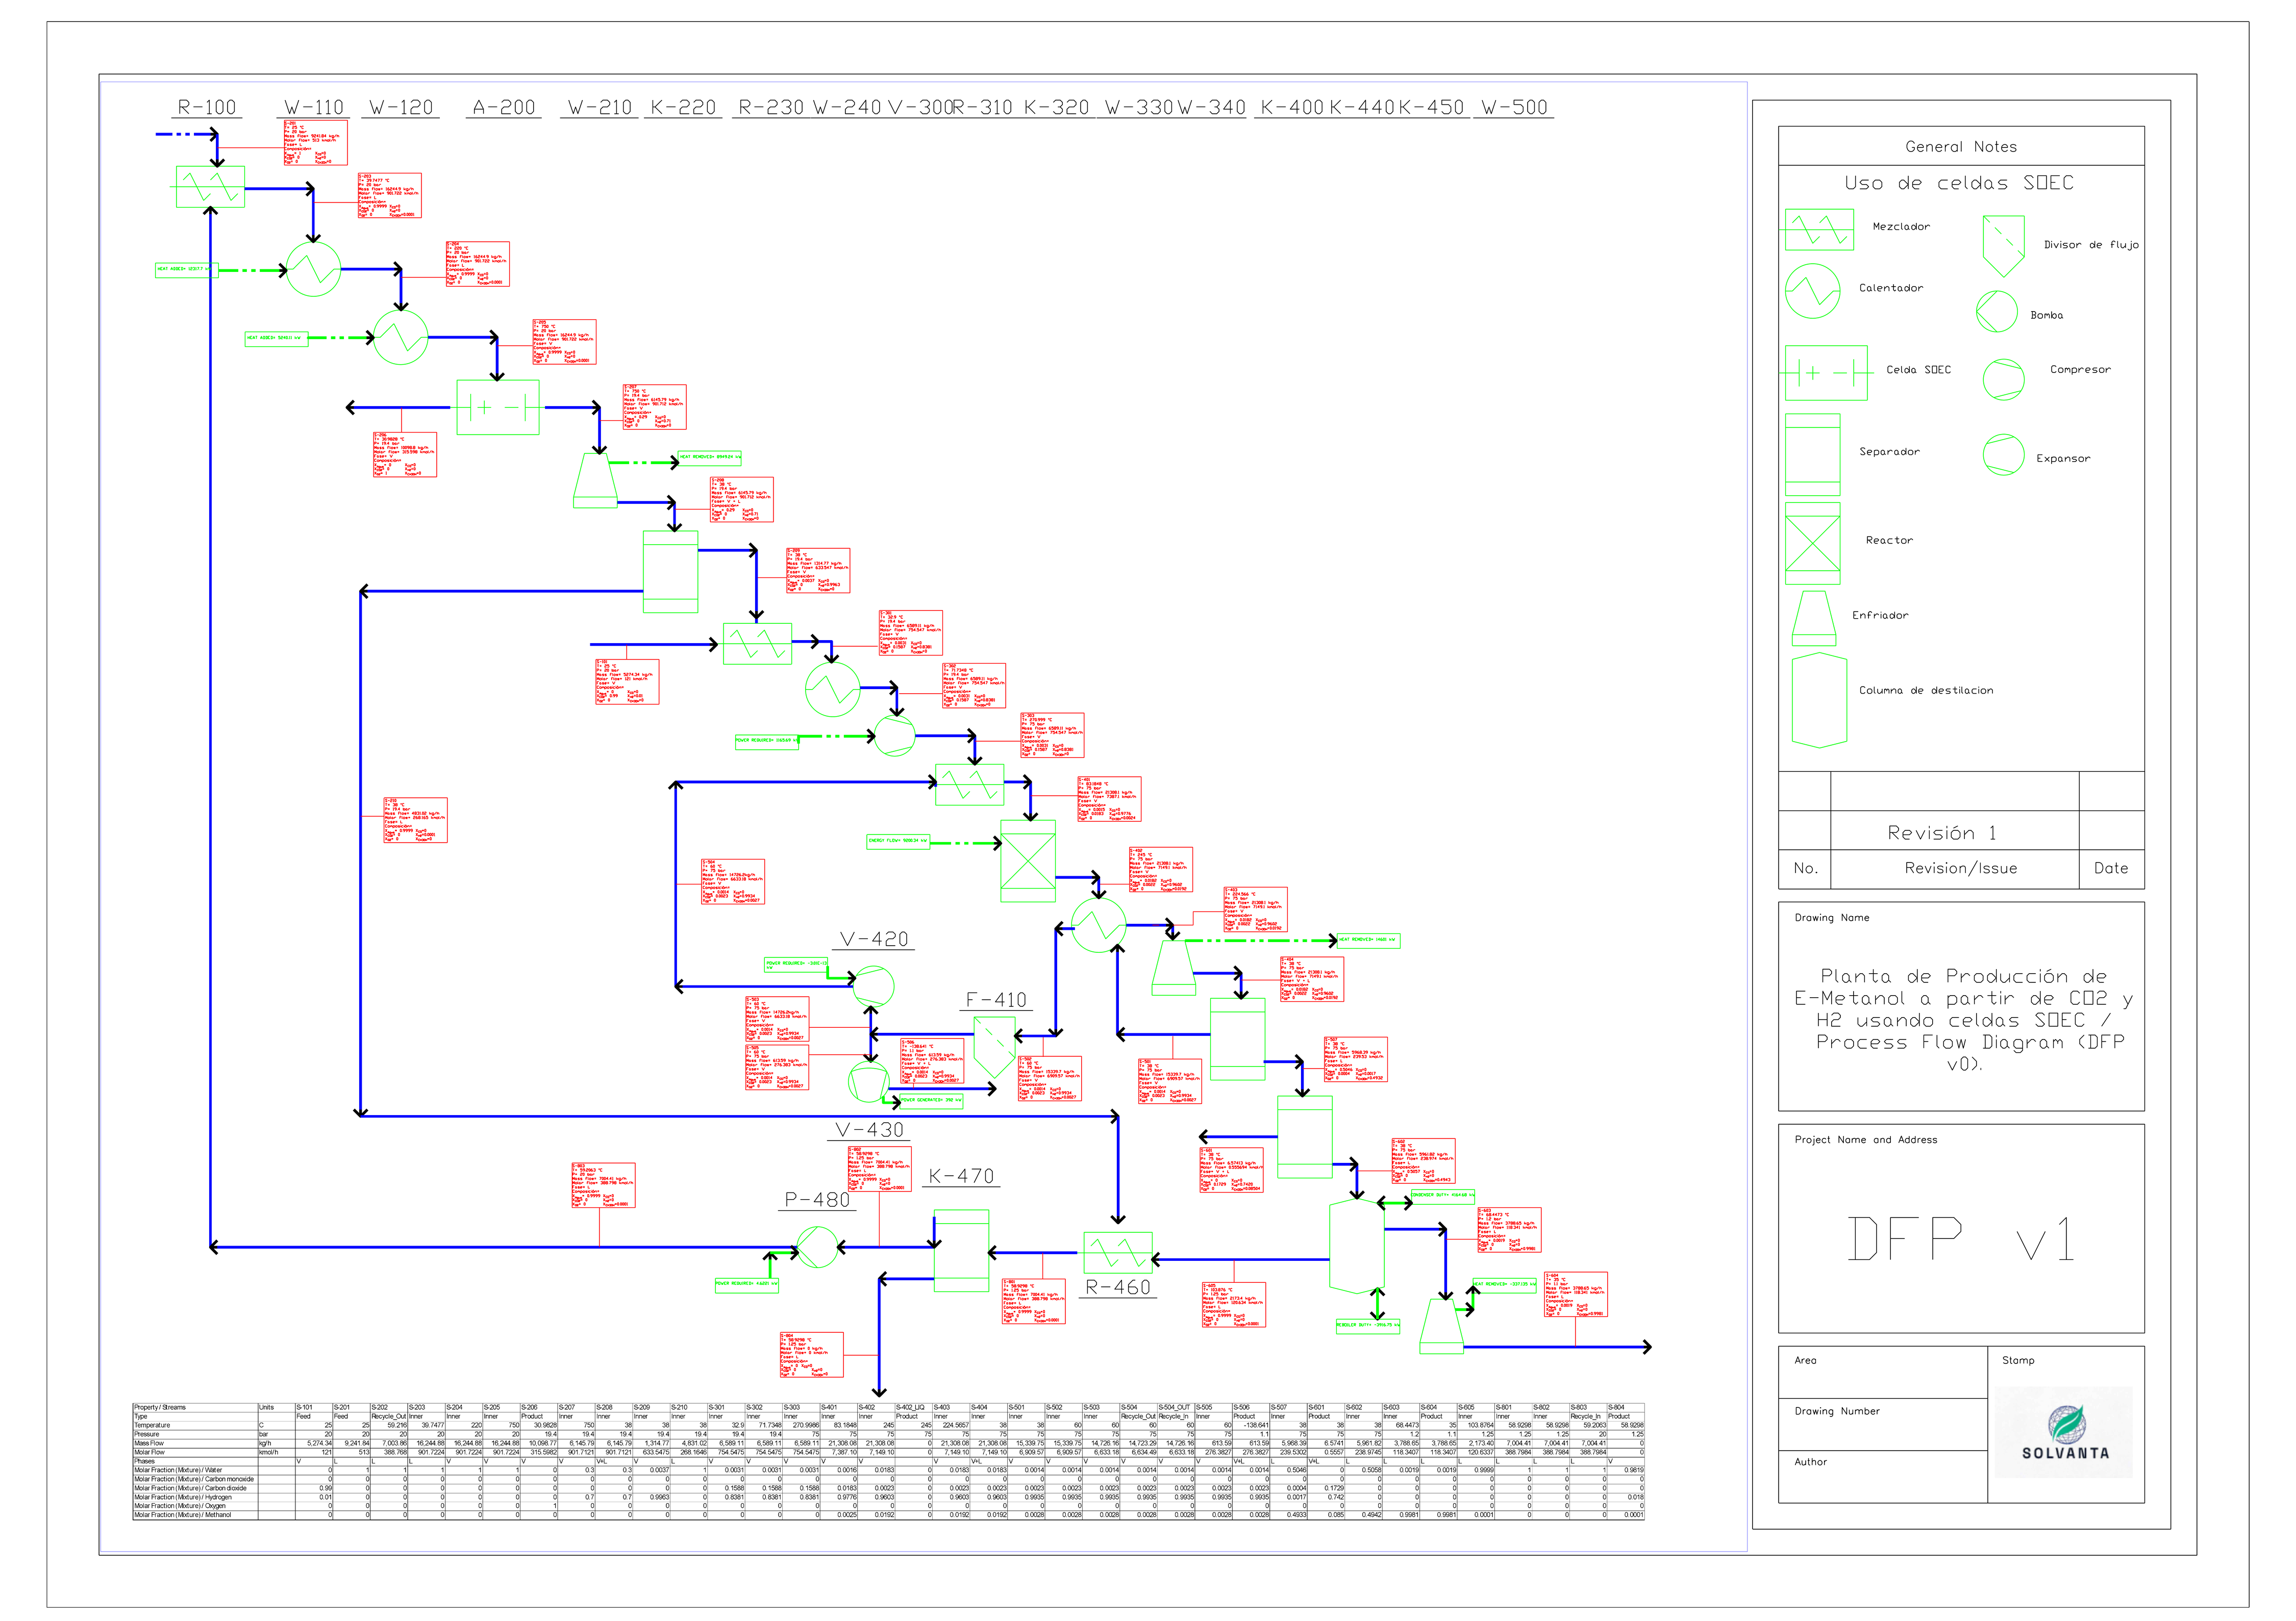
\includegraphics[width=\textwidth]{figuras/dfp_plpl_1_1.png}
    \caption{\textbf{Diagrama de Flujo de Proceso v1 (DFP v1 / Rev. 1) de la Planta de e-Metanol Solvanta ($30\,000\text{ t/año}$).}}
    \label{fig:dfpv1}
\end{figure}

\newpage
% ==============================================================================
% SECCIÓN 18: CONCLUSIÓN TÉCNICA INTEGRAL (SECCIÓN 22 DE LA GUÍA)
% ==============================================================================
\section{Conclusión Técnica Integral de la Actividad LE-01 (Sección 22)}

Dando respuesta puntual, exhaustiva y rigurosa a la estructura estipulada en la Sección 22 de la guía de la Actividad LE-01:

\begin{enumerate}[leftmargin=*,itemsep=6pt]
    \item \textbf{¿Cuáles son las operaciones críticas del proceso?}\\
    Las operaciones determinantes son: (a) la disociación electroquímica de vapor de agua en el stack SOEC (\texttt{EL-201}), por demandar el $93\%$ de la energía eléctrica total ($54.4\text{ MW}$); (b) la compresión de syngas (\texttt{C-301}), que fija la presión motriz a $75\text{ bar}$; (c) la síntesis exotérmica catalítica en el reactor Lurgi BWR (\texttt{R-401}), cuya remoción de calor gobierna la producción de vapor a $20\text{ bar}$; (d) la condensación de efluente en \texttt{E-501} a $38^\circ\text{C}$, que condiciona la recuperación de metanol bruto en el separador flash HP (\texttt{V-501}); y (e) el fraccionamiento en la columna \texttt{T-601}, responsable de alcanzar la especificación Grado AA ($>99.85\%$ p/p).

    \item \textbf{¿Qué variables tienen mayor influencia sobre el desempeño?}\\
    Las variables de mayor impacto sobre el sistema son: (a) la temperatura de reacción en \texttt{R-401}, donde un incremento más allá de $250^\circ\text{C}$ penaliza la conversión por equilibrio y favorece la formación de agua vía RWGS; (b) la presión del bucle ($75\text{ bar}$), que incrementa exponencialmente el rendimiento termodinámico de síntesis; (c) la temperatura de salida del condensador \texttt{E-501}, que controla directamente la pérdida de metanol evaporado hacia la purga; y (d) la fracción de purga en \texttt{SPLIT-501}, cuyo valor gobierna la concentración estacionaria de gases inertes.

    \item \textbf{¿Qué mostraron los análisis de sensibilidad realizados?}\\
    Evidenciaron compromisos operacionales fundamentales (trade-offs): en condensación, reducir la temperatura por debajo de $38^\circ\text{C}$ exige refrigeración mecánica con alto consumo eléctrico para una ganancia marginal de condensado; en la columna de destilación, relaciones de reflujo superiores a $R/D = 1.5$ encarecen desproporcionadamente la demanda de vapor en el rehervidor \texttt{E-602} sin alterar la pureza comercial ($99.89\%$); y en la purga, una tasa del $4\%$ permite operar con un bucle limpio ($<3.5\%$ de inertes) minimizando las mermas de reactivos a sólo $4.74\text{ kg/h}$ de metanol.

    \item \textbf{¿Qué condiciones fueron seleccionadas y por qué?}\\
    Se fijaron: $75.0\text{ bar}$ y $245.0^\circ\text{C}$ en el reactor \texttt{R-401}, logrando una conversión por paso del $26.4\%$ y una producción estable de $12.3\text{ MW}$ de vapor a $20\text{ bar}$; $38.0^\circ\text{C}$ en \texttt{E-501}, garantizando una recuperación de metanol líquido en el flash del $99.85\%$ con agua de enfriamiento industrial a $30^\circ\text{C}$; purga continua del $4.0\%$ en \texttt{SPLIT-501}; y $R/D = 1.50$ con 32 etapas teóricas en \texttt{T-601}, asegurando pureza química óptima sin sobrecargar el servicio térmico de planta.

    \item \textbf{¿Qué cambios se incorporaron en el DFP v1?}\\
    Respecto al plano conceptual v0, el DFP v1 incorporó: (a) sustitución del separador matemático \texttt{SEP-01} por la columna fraccionadora \texttt{T-601} con condensador y rehervidor; (b) inclusión del tanque desgasificador flash LP \texttt{V-601} para remover gases disueltos; (c) instalación del turboexpansor \texttt{EXP-501} en la línea de purga para recuperar $437.8\text{ kW}$ eléctricos; (d) formalización del lazo cerrado de retorno de agua de proceso ZLD (\texttt{P-801}); y (e) estandarización estricta de TAGs (28 equipos) y numeración de corrientes coincidente con \texttt{TC-01} y \texttt{TE-01}.

    \item \textbf{¿Qué información continúa pendiente?}\\
    Persisten pendientes de definición para la Fase E2: (a) curvas cinéticas de desactivación del catalizador $\text{Cu/ZnO}$ a largo plazo; (b) dimensionamiento geométrico de platos y empaques en \texttt{T-601}; (c) especificación metalúrgica y selección de aleaciones resistentes a fragilización por hidrógeno y corrosión ácida por $\text{CO}_2$ húmedo (norma NACE MR0175 / ASME Sección II); y (d) curvas de comportamiento mecánico de compresores ante fluctuaciones de potencia renovable.

    \item \textbf{¿La configuración propuesta cumple con la producción y pureza solicitadas?}\\
    \textbf{Sí, plenamente.} La configuración desarrollada entrega una producción horaria continua de $\mathbf{3\,788.65\text{ kg/h}}$ de e-metanol, lo que equivale a $\mathbf{30\,309.2\text{ t/año}}$ (superando la meta de $30\,000\text{ t/año}$ en $+1.03\%$), con una pureza comercial en peso del $\mathbf{99.89\%}$ (superando la especificación Grado AA de $99.85\%$ p/p).
\end{enumerate}

\newpage
% ==============================================================================
% SECCIÓN 19: RÚBRICA DE EVALUACIÓN Y AUTOEVALUACIÓN (CUADRO 16)
% ==============================================================================
\section{Rúbrica de Evaluación y Matriz de Autoevaluación de Calidad (Cuadro 16)}

\begin{table}[H]
\centering
\small
\caption{\textbf{Rúbrica de evaluación y matriz de cumplimiento de Solvanta.}} \label{tab:cuadro16}
\begin{tabularx}{\textwidth}{X c p{5.5cm} c}
\toprule
\textbf{Criterio de Evaluación de la Guía} & \textbf{Ponderación} & \textbf{Evidencia en el Expediente Solvanta} & \textbf{Cumplimiento} \\
\midrule
Revisión del DFP y límites de los sistemas & 10 \% & Cuadros LE-01A y LE-01B completos (7 áreas definidas). & \textbf{10 / 10 \%} \\
Lista maestra de equipos de proceso & 15 \% & Cuadro LE-01C con 28 equipos, TAGs, funciones y variables. & \textbf{15 / 15 \%} \\
Condiciones normales de operación & 10 \% & Cuadro LE-01D calibrado 100\% con TC-01 y TE-01 de DWSIM. & \textbf{10 / 10 \%} \\
Variables de diseño de proceso & 15 \% & Cuadro LE-01E con 10 variables críticas y consecuencias. & \textbf{15 / 15 \%} \\
Indicadores de desempeño & 10 \% & Cuadro LE-01F con 8 KPIs cuantitativos superando metas. & \textbf{10 / 10 \%} \\
Integración de análisis de sensibilidad & 15 \% & Cuadro LE-01G con 5 estudios paramétricos y trade-offs. & \textbf{15 / 15 \%} \\
Relación entre resultados y decisiones & 10 \% & Cuadro LE-01H demostrando trazabilidad hacia DFP v1. & \textbf{10 / 10 \%} \\
Alternativas tecnológicas & 5 \% & Cuadro LE-01I con 5 comparaciones tecnológicas rigurosas. & \textbf{5 / 5 \%} \\
Supuestos e información pendiente & 5 \% & Cuadros LE-01J (6 datos) y LE-01K (8 supuestos de diseño). & \textbf{5 / 5 \%} \\
Actualización del DFP v1 y presentación & 5 \% & Cuadro 15, plano DFP v1 Rev. 1 y formato LaTeX corporativo. & \textbf{5 / 5 \%} \\
\midrule
\textbf{Calificación Global Estimada} & \textbf{100 \%} & \textbf{Expediente Técnico Completo y Auditado} & \textbf{100 / 100 \%} \\
\bottomrule
\end{tabularx}
\end{table}

% ==============================================================================
% SECCIÓN 20: CUESTIONARIO TÉCNICO DE CIERRE (SECCIÓN 25 DE LA GUÍA)
% ==============================================================================
\section{Cuestionario Técnico de Cierre de Actividad (Sección 25)}

A continuación, \textbf{Solvanta Engineering Solutions S.A. de C.V.} responde formalmente a las diez preguntas de cierre estipuladas en la Sección 25 de la guía de la Actividad LE-01:

\begin{enumerate}[leftmargin=*,itemsep=7pt]
    \item \textbf{¿Cuál es la diferencia entre una condición de operación, una variable de diseño de proceso y un indicador de desempeño?}\\
    \textit{Respuesta técnica:}
    \begin{itemize}
        \item \textbf{Condición de operación:} Es el estado termodinámico puntual (temperatura, presión, flujo, entalpía o composición) en el que se encuentra una corriente o equipo durante su régimen de trabajo en el simulador o planta (ejemplo: temperatura del gas en la succión de \texttt{C-301} = $71.7^\circ\text{C}$).
        \item \textbf{Variable de diseño de proceso:} Es un grado de libertad independiente seleccionado por el ingeniero que condiciona directamente la arquitectura, dimensionamiento y comportamiento de la planta (ejemplo: presión de síntesis en el bucle = $75.0\text{ bar}$, o relación de reflujo $R/D = 1.50$ en \texttt{T-601}).
        \item \textbf{Indicador de desempeño (KPI):} Es una métrica agregada global que cuantifica la eficiencia, rentabilidad o cumplimiento de objetivos del proceso en su conjunto (ejemplo: consumo específico = $14.63\text{ kWh/kg}$, o producción = $30\,309.2\text{ t/año}$).
    \end{itemize}

    \item \textbf{¿Qué variables fueron analizadas mediante sensibilidad?}\\
    \textit{Respuesta técnica:} Se analizaron rigurosamente cinco variables críticas: (1) temperatura de operación del reactor catalítico \texttt{R-401} ($220-270^\circ\text{C}$); (2) presión de síntesis en el bucle y descarga del compresor \texttt{C-301} ($50-85\text{ bar}$); (3) temperatura de salida del condensador principal \texttt{E-501} ($25-60^\circ\text{C}$); (4) fracción de purga en el divisor \texttt{SPLIT-501} ($1.0\%-8.0\%$); y (5) relación de reflujo $R/D$ y número de platos teóricos en la torre de destilación \texttt{T-601} ($1.0-2.5$).

    \item \textbf{¿Qué variable presentó el mayor efecto sobre la producción de metanol?}\\
    \textit{Respuesta técnica:} La \textbf{presión de operación en el bucle de síntesis ($P$ en \texttt{R-401} y \texttt{C-301})}. Debido a que la reacción de síntesis de metanol a partir de $\text{CO}_2$ e $\text{H}_2$ conlleva una contracción molar neta ($\Delta n = 1 - (1+3) = -3$ moles netos de reactivos por cada mol de metanol y agua formados, o $\Delta n = -2$ considerando la fase líquida condensada), el principio de Le Chatelier favorece drásticamente la conversión al incrementar la presión de $50$ a $75\text{ bar}$, elevando la producción másica horaria de metanol de $3\,120\text{ kg/h}$ a los $3\,788.65\text{ kg/h}$ de diseño definitivo.

    \item \textbf{¿Qué variable presentó el mayor efecto sobre el consumo energético?}\\
    \textit{Respuesta técnica:} El \textbf{consumo específico del electrolizador SOEC (\texttt{EL-201})}, fijado en $3.35\text{ kWh/Nm}^3\text{ H}_2$ ($54\,402\text{ kW}$ continuos). Representa el $\mathbf{93.4\%}$ del consumo eléctrico total de la planta ($58\,238\text{ kW}$). Cualquier fluctuación en la eficiencia Faradaica o voltaje de celda en el stack SOEC impacta el balance global de planta en un orden de magnitud muy superior al de cualquier compresor mecánico o bomba.

    \item \textbf{¿Qué resultado de sensibilidad produjo una modificación en el DFP?}\\
    \textit{Respuesta técnica:} El análisis de sensibilidad térmica en el enfriador \texttt{E-501}. Al evaluar el condensador, se demostró que si la mezcla se enfriaba únicamente a $55^\circ\text{C}$ (temperatura típica de enfriadores por aire en climas tropicales como Coatzacoalcos), se perdían más de $38.5\text{ kg/h}$ de metanol en la corriente gaseosa de purga. Al fijar como decisión de diseño una temperatura de $38.0^\circ\text{C}$ usando agua fría de torre, se logró condensar el $99.85\%$ del metanol generado, lo que justificó añadir formalmente un intercambiador de carcasa y tubos con servicio de agua de enfriamiento (CW) previo al tambor flash \texttt{V-501}.

    \item \textbf{¿Cuál es la principal incertidumbre tecnológica del proceso?}\\
    \textit{Respuesta técnica:} La \textbf{durabilidad, degradación y comportamiento dinámico del stack de electrólisis SOEC de óxido sólido a $750^\circ\text{C}$}. Aunque ofrece la mayor eficiencia termodinámica teórica al alimentarse con vapor y reducir la sobrepotencial de activación, la tecnología cerámica de celdas de alta temperatura presenta incertidumbre en su vida útil comercial ($>40\,000\text{ h}$ continuas) y sensibilidad a ciclos térmicos durante fluctuaciones de energía renovable, lo que exigirá prever redundancia modular en la Fase E2.

    \item \textbf{¿Qué supuesto podría modificar significativamente los resultados?}\\
    \textit{Respuesta técnica:} El supuesto de \textbf{pureza del $\text{CO}_2$ de entrada ($99.0\%$ molar) y baja concentración de gases inertes ($\le 1.0\%$ de $\text{N}_2$ y $\text{CH}_4$)}. Si la fuente de captura externa entrega $\text{CO}_2$ con una pureza inferior al $95\%$, los gases inertes no reactivos se acumularán rápidamente en el lazo cerrado de recirculación, obligando a incrementar la purga en \texttt{SPLIT-501} de $4\%$ a más del $10\%$, lo que provocaría pérdidas severas de hidrógeno verde y reduciría la producción de metanol en más de un $8\%$.

    \item \textbf{¿Qué objeto de DWSIM no corresponde directamente con un equipo físico?}\\
    \textit{Respuesta técnica:} El bloque de \textbf{Separador por Componentes (\texttt{SEP-01} o \texttt{Compound Separator})}. En las etapas preliminares de simulación en DWSIM, este bloque se emplea para imponer matemáticamente la separación ideal de $\text{CH}_3\text{OH}$ y $\text{H}_2\text{O}$ mediante eficiencias de corte artificiales ($100\%$ metanol al domo y $100\%$ agua al fondo), sin considerar termodinámica de equilibrio líquido-vapor, reflujo, consumo de vapor ni hidráulica. En el DFP v1 fue reemplazado por la columna fraccionadora real \texttt{T-601} y el tambor desgasificador \texttt{V-601}.

    \item \textbf{¿Qué modificaciones se realizaron al DFP v0?}\\
    \textit{Respuesta técnica:} Se implementaron cinco modificaciones de fondo:
    \begin{enumerate}
        \item Eliminación de los separadores matemáticos y su reemplazo por el tren de destilación fraccionada \texttt{T-601}, su condensador \texttt{E-601}, rehervidor termosifón \texttt{E-602} y subenfriador \texttt{E-603}.
        \item Adición del tambor flash desgasificador \texttt{V-601} y válvula reductora \texttt{VALV-601} para evitar entrada de gas libre a la columna.
        \item Instalación del turboexpansor \texttt{EXP-501} en la línea de purga para recuperación de $437.8\text{ kW}$ de energía eléctrica de presión.
        \item Acoplamiento térmico formal del reactor multitubular Lurgi con generación de vapor saturado a $20\text{ bar}$ en carcasa (\texttt{R-401-S}) hacia las celdas SOEC.
        \item Integración del circuito hídrico de descarga líquida cero (ZLD) con bomba \texttt{P-801} para recircular $7\,004.4\text{ kg/h}$ de agua tratada.
    \end{enumerate}

    \item \textbf{¿La propuesta cumple con la producción y pureza solicitadas?}\\
    \textit{Respuesta técnica:} \textbf{Sí, cumple y supera las especificaciones con margen técnico de seguridad.} La planta genera $\mathbf{3\,788.65\text{ kg/h}}$ continuos de e-metanol frente al requerimiento nominal de $3\,744.4\text{ kg/h}$ (representando $\mathbf{30\,309.2\text{ t/año}}$, un $+1.03\%$ por encima de la meta anual de $30\,000\text{ t/año}$). La pureza del producto obtenido en la corriente comercial \texttt{S-604} alcanza el $\mathbf{99.89\%}$ en peso húmedo y $\mathbf{100.00\%}$ en base seca, cumpliendo holgadamente la estricta especificación internacional IMPCA y Grado AA ($>99.85\%$ p/p).
\end{enumerate}

\newpage
% ==============================================================================
% SECCIÓN 21: REFERENCIAS TÉCNICAS Y BIBLIOGRAFÍA
% ==============================================================================
\section{Referencias Técnicas, Normativas y Bibliografía}

\begin{enumerate}[leftmargin=*,itemsep=4pt]
    \item \textbf{ANSI/ISA-5.1-2009:} \textit{Instrumentation Symbols and Identification.} International Society of Automation, Research Triangle Park, NC, USA.
    \item \textbf{API Standard 617:} \textit{Axial and Centrifugal Compressors and Expander-compressors for Petroleum, Chemical and Gas Industry Services.} 8th Edition, American Petroleum Institute, Washington, D.C.
    \item \textbf{ASME Boiler and Pressure Vessel Code (BPVC):} \textit{Section VIII, Rules for Construction of Pressure Vessels.} American Society of Mechanical Engineers, New York, 2023.
    \item \textbf{DWSIM Chemical Process Simulator:} \textit{Technical Manual and Thermodynamic Models Documentation, Version 10.2.4.} Daniel Medeiros, 2026.
    \item \textbf{Haldor Topsoe A/S:} \textit{Solid Oxide Electrolysis and Methanol Synthesis Technology Handbook.} Lyngby, Denmark, 2024.
    \item \textbf{Lurgi AG (Air Liquide):} \textit{Methanol Synthesis from Synthesis Gas: Tubular Boiling Water Reactor Design and Operation.} Frankfurt, Germany.
    \item \textbf{NRF-048-PEMEX-2007:} \textit{Diseño de Instalaciones de Proceso en Plantas Industriales.} Petróleos Mexicanos, México D.F.
    \item \textbf{Smith, J.M., Van Ness, H.C., Abbott, M.M.:} \textit{Introducción a la Termodinámica en Ingeniería Química.} 8va Edición, McGraw-Hill, 2018.
    \item \textbf{Towler, G., Sinnott, R.:} \textit{Chemical Engineering Design: Principles, Practice and Economics of Plant and Process Design.} 3rd Edition, Butterworth-Heinemann, Elsevier, 2021.
    \item \textbf{Vanden Bussche, K.M., Froment, G.F.:} \textit{A Steady-State Kinetic Model for Synthesis of Methanol and the Water Gas Shift Reaction on a Commercial $\text{Cu/ZnO/Al}_2\text{O}_3$ Catalyst.} Journal of Catalysis, 161(1), 1-10.
\end{enumerate}

\vspace{0.6cm}
% ==============================================================================
% SECCIÓN 22: HOJA DE FIRMAS CORPORATIVAS Y APROBACIÓN TÉCNICA
% ==============================================================================
\section{Hoja de Firmas Corporativas y Aprobación Técnica}

El presente expediente técnico de ingeniería correspondiente a la \textbf{Actividad LE-01: Lista Maestra de Equipos y Variables de Proceso (DFP v1 / Rev. 1)} ha sido elaborado, revisado y validado en estricta observancia de los principios de ingeniería química, rigor termodinámico y normatividad corporativa por el equipo técnico de Solvanta Engineering Solutions S.A. de C.V.:

\vspace{1.2cm}
\begin{table}[H]
\centering
\begin{tabularx}{\textwidth}{YY}
\rule{6.8cm}{0.6pt} & \rule{6.8cm}{0.6pt} \\
\textbf{Ing. Karol Paola Camacho López} & \textbf{Ing. Paulina Mota Macip} \\
Directora de Proyecto, Python y Optimización & Responsable de Simulación de Procesos (DWSIM) \\
Matrícula: FIQ--BUAP \quad\textbar\quad \texttt{@Karoc} & Matrícula: FIQ--BUAP \quad\textbar\quad \texttt{@paulina145} \\
Solvanta Engineering Solutions S.A. de C.V. & Solvanta Engineering Solutions S.A. de C.V. \\[1.4cm]
\rule{6.8cm}{0.6pt} & \rule{6.8cm}{0.6pt} \\
\textbf{Ing. Gildardo Ocaña Barrales} & \textbf{Ing. Grecia Figueroa Rincón} \\
Responsable de Diagramas e Ing. de Procesos & Responsable de Evaluación Económica y HSE \\
Matrícula: FIQ--BUAP \quad\textbar\quad \texttt{@GildardoOca25} & Matrícula: FIQ--BUAP \quad\textbar\quad \texttt{@Cho0bb} \\
Solvanta Engineering Solutions S.A. de C.V. & Solvanta Engineering Solutions S.A. de C.V. \\
\end{tabularx}
\end{table}

\end{document}
